%%%%%%%%%%%%%%%%%%%%%%%%%%%%%%%%%%%%%%%%%%%%%%%%%%%%%%%%%%%%%%%%%%%%%%%%%%%
% PFC/Tesis Latex Template
%%%%%%%%%%%%%%%%%%%%%%%%%%%%%%%%%%%%%%%%%%%%%%%%%%%%%%%%%%%%%%%%%%%%%%%%%%%
\documentclass[svgnames,spanish,openright]{book}
%\documentclass[english,openright]{book}
%\documentclass[11pt,english,twoside,openright]{book}

%\usepackage[a4,cam,center]{crop}
%\crop[font=\upshape\mdseries\small\textsf]

\usepackage[latin1]{inputenc} % Para poder escribir con acentos y �.
\usepackage[T1]{fontenc}      % Para que haga bien la ``hyphenation''. No
                              % usar si no es necesario, porque ralentiza muchisimo la compilaci�n.
\usepackage{ae}               % Para que todas las fuentes sean Type1, y ninguna Type3.

\usepackage[spanish, english]{babel}

% Use this if you want to include pdf files in the final document
\usepackage[final]{pdfpages}

% Use this if you want to delete headers and footers in empty pages
\usepackage{emptypage}

%\usepackage[nottoc]{tocbibind}
\usepackage{tocbibind}

% To draw rectagles in tfm cover
\usepackage{tikz}

\usepackage{listings}
\usepackage{longtable}
\usepackage{afterpage}

\usepackage{xspace}
\usepackage{verbatim}
\usepackage{moreverb}
\usepackage{multicol}
\usepackage{amsmath}
\usepackage{eurosym}
\usepackage{subfigure}
\usepackage{multirow}
\usepackage{fancyhdr}
\usepackage{makeidx}
\usepackage{rotating}
\usepackage{supertabular}
\usepackage{hhline}
\usepackage{array}
\usepackage[noadjust]{cite}      % Written by Donald Arseneau
                        % V1.6 and later of IEEEtran pre-defines the format
                        % of the cite.sty package \cite{} output to follow
                        % that of IEEE. Loading the cite package will
                        % result in citation numbers being automatically
                        % sorted and properly "ranged". i.e.,
                        % [1], [9], [2], [7], [5], [6]
                        % (without using cite.sty)
                        % will become:
                        % [1], [2], [5]--[7], [9] (using cite.sty)
                        % cite.sty's \cite will automatically add leading
                        % space, if needed. Use cite.sty's noadjust option
                        % (cite.sty V3.8 and later) if you want to turn this
                        % off. cite.sty is already installed on most LaTeX
                        % systems. The latest version can be obtained at:
                        % http://www.ctan.org/tex-archive/macros/latex/contrib/supported/cite/


\usepackage{color}

%\usepackage[authoryear]{natbib}
% \makeatletter
% \let\NAT@parse\undefined
% \makeatother
% \usepackage{natbib}

\usepackage{geometry}
\geometry{verbose,a4paper,tmargin=2.5cm,bmargin=2.5cm,lmargin=2.5cm,rmargin=2.5cm}
%\geometry{paperwidth=210mm,paperheight=297mm}

\usepackage[
ps2pdf,                %%% hyper-references for ps2pdf
bookmarks=true,%                   %%% generate bookmarks ...
bookmarksnumbered=true,            %%% ... with numbers
hypertexnames=false,               %%% needed for correct links to
                                %%% figures!!!
%hypertexnames=true,               %%% needed for correct links on pagebackrefs!!!
breaklinks=true,                   %%% breaks lines, but links are very small
%pagebackref=true,
%linktocpage=true,                 %%% enlace en el numero de p�gina.
linktoc=all,
colorlinks=true,
linkcolor=azul,    
citecolor=verde,
urlcolor=azul,                     %%% texto  con color
linkbordercolor={0 0 1},           %%% blue frames around links
pdfborder={0 0 112.0}              %%% border-width of frames 
]{hyperref}                        %%% will be multiplied with 0.009 by ps2pdf


% Para numerar las \subsubsection
\setcounter{secnumdepth}{5}
%para hacer que las \subsubsection aparezcan en el indice
\setcounter{tocdepth}{5}
%\setcounter{lofdepth}{2}
\setcounter{table}{1}
\setcounter{figure}{1}
\setcounter{secnumdepth}{4}


\setlength{\parskip}{1ex plus 0.5ex minus 0.2ex}


\usepackage{multirow}

\usepackage{setspace}
% \renewcommand{\baselinestretch}{10}
\newcommand{\mycaptiontable}[1]{
\begin{spacing}{0.6}
  %\vspace{0.5cm}
  \begin{quote}
    %\begin{center}
            {{Table} \thechapter.\arabic{table}: #1}
    %\end{center}
  \end{quote}
  %\vspace{1cm}
  \end{spacing}
  \stepcounter{table}
}

\newcommand{\mycaptionfigure}[1]{
  %\vspace{0.5cm}
  \begin{spacing}{0.6}
  \begin{quote}
    %\begin{center}
            {{Figure} \thechapter.\arabic{figure}: #1}
    %\end{center}
  \end{quote}
  %\vspace{1cm}
  \end{spacing}
  \stepcounter{figure}
}

% \newlength{\myVSpace}% the height of the box
% \setlength{\myVSpace}{0ex}% the default, 
% \newcommand\xstrut{\raisebox{-.5\myVSpace}% symmetric behaviour, 
%   {\rule{0pt}{\myVSpace}}%
% }

\usepackage{amsmath}

\usepackage{courier}

%***************************************************************************
%***************************************************************************
%***************************************************************************
\usepackage{multirow}
\usepackage{rotating}
\usepackage{setspace, amssymb, amsmath, epsfig, multirow, colortbl, tabularx, subfigure}%
% For acronym package:
% If footnote is specified, text will be included in a footnote
% If printonlyused is specified, only used acronyms will be included
% I use the acronym sty under the sty directory as I needed the newest version
%\usepackage[footnote,printonlyused,withpage]{acronym} 
%\usepackage[printonlyused]{sty/acronym}

% Mejor que el acronym es glossaries
\usepackage[acronym,shortcuts,nomain]{glossaries}

% ifthen to allow using language dependent settings
\usepackage{ifthen}

\newcommand{\clearemptydoublepage}{\newpage{\pagestyle{empty}\cleardoublepage}}


\pagestyle{fancy}

% Pantone 160
%\definecolor{headingPortadaTFM}{RGB}{158,84,10}
% Pantone 160C (this is supposed to be the correct one, but it looks horrible in screen)
%\definecolor{headingPortadaTFM}{RGB}{161,86,28}
% Captured color in screen (this looks ok on screen)
\definecolor{headingPortadaTFM}{RGB}{152,118,52}
\definecolor{textoHeadingPortadaTFM}{RGB}{208,205,102}

\definecolor{azul}{rgb}{0,0,1}
\definecolor{verde}{rgb}{0,0.5,0}
\definecolor{rojo}{rgb}{1,0,0}
\definecolor{cyan}{rgb}{0,0.75,0.75}
\definecolor{magenta}{rgb}{0.75,0,0.75}
\definecolor{amarillo}{rgb}{0.75,0.75,0}
\definecolor{gris}{rgb}{0.25,0.25,0.25}
\definecolor{r}{rgb}{0,0,1}
\definecolor{g}{rgb}{0,1,0}
\definecolor{b}{rgb}{1,0,0}
\definecolor{c}{rgb}{0,1,1}
\definecolor{m}{rgb}{1,0,1}
\definecolor{y}{rgb}{1,1,0}
\definecolor{w}{rgb}{1,1,1}
\definecolor{k}{rgb}{0,0,0}
\definecolor{azulE}{rgb}{0,0.3984,0.5977}
\definecolor{amarilloE}{rgb}{0.9961,0.7969,0}
\definecolor{blanco}{rgb}{1,1,1}
\definecolor{burdeos}{rgb}{1,0,0.95}


\providecommand\phantomsection{}
\onehalfspacing
\sloppy  %better line breaks

\renewcommand{\chaptermark}[1]{\markboth{\chaptername\ \thechapter.\ #1}{}}
\renewcommand{\sectionmark}[1]{\markright{\thesection\ #1}{}}



\fancyhf{}

\fancyhead[LE,RO]{\bfseries\thepage}
\fancyhead[LO]{\bfseries\rightmark}
\fancyhead[RE]{\bfseries\leftmark}

\renewcommand{\headrulewidth}{0.5pt}
\renewcommand{\footrulewidth}{0pt}
\addtolength{\headheight}{3.5pt}
\fancypagestyle{plain}{\fancyhead{}  
  \renewcommand{\headrulewidth}{0pt}}

%\makeglossaries

\fancypagestyle{myplain}
{
  \fancyhf{}
  \renewcommand\headrulewidth{0pt}
  \renewcommand\footrulewidth{0pt}
  \fancyfoot[C]{\thepage}
}

% To set background image in TFMs front and back pages
\usepackage[pages=some]{sty/background}

\backgroundsetup{ scale=1, angle=0, opacity=.1, color=pink,
  contents={\includegraphics[width=.7\paperwidth]{logos/logoEPS-UAH.jpg}}, vshift=-50pt,  hshift=0pt }

\makeatletter
\newcommand*{\cleartoleftpage}{%
  \clearpage
    \if@twoside
    \ifodd\c@page
      \hbox{}\newpage
      \if@twocolumn
        \hbox{}\newpage
      \fi
    \fi
  \fi
}
\makeatother
    % All definitions, packages, etc.

%%%%%%%%%%%%%%%%%%%%%%%%%%%%%%%%%%%%%%%%%%%%%%%%%%%%%%%%%%%%%%%%%%%%%%%%%%%
% You can define your own commands in this file

% This one is to define a specific format for english text in a Spanish
% document
\DeclareRobustCommand{\texten}[1]{\textit{#1}}

% Various examples
\newcommand{\circulo}{\large $\circ$}
\newcommand{\asterisco}{$\ast$}
\newcommand{\cuadrado}{\tiny $\square$}
\newcommand{\triangulo}{\scriptsize $\vartriangle$}
\newcommand{\triangv}{\scriptsize $\triangledown$}
\newcommand{\diamante}{\large $\diamond$}

\newcommand{\new}[1]{\textcolor{magenta}{#1 }}
\newcommand{\argmax}[1]{\underset{#1}{\operatorname{argmax}}}
\newcommand{\argmaxmax}[1]{\underset{#1}{\operatorname{argmaxmax}}}


  % Include your own commands here. EDIT
                               % IT!

\newboolean{english}

\setboolean{english}{false} % Use this to set some Spanish modifications
%\setboolean{english}{true} 
 % This defines the value of the boolean
                               % english. EDIT IT! Setting the variable
                               % will automatically adjust some defaults

% Define a new glossary type for symbols used in equations
\newglossary[slg]{symbols}{sym}{sbl}{List of Symbols}


\makeglossaries
  % EDIT IT to include your glossaries!

%%%%%%%%%%%%%%%%%%%%%%%%%%%%%%%%%%%%%%%%%%%%%%%%%%%%%%%%%%%%%%%%%%%%%%%%%%%
% Info for the pdf file
%%%%%%%%%%%%%%%%%%%%%%%%%%%%%%%%%%%%%%%%%%%%%%%%%%%%%%%%%%%%%%%%%%%%%%%%%%%
\hypersetup
{
  pdfauthor={Nombre y apellidos del autor <autor@depeca.uah.es>},
  pdftitle={T�tulo del proyecto},
  pdfsubject={Proyecto Fin de Carrera},
  pdfkeywords={pfc template, latex document},
  pdfcreator={LaTeX with hyperref package},
  pdfproducer={rubber},
  pdffitwindow={true}
}
     % This sets the general information kept
                               % in the pdf file. EDIT IT!

% ruta de las im�genes
\graphicspath{{./logos/}{./results/}{./diagrams/}}

%%%%%%%%%%%%%%%%%%%%%%%%%%%%%%%%%%%%%%%%%%%%%%%%%%%%%%%%%%%%%%%%%%%%%%%%%%%
% Let's start with the real stuff
%%%%%%%%%%%%%%%%%%%%%%%%%%%%%%%%%%%%%%%%%%%%%%%%%%%%%%%%%%%%%%%%%%%%%%%%%%%
\begin{document}

% Now start text and numbering for toc, list of tables/figures,...
\frontmatter

% Set Language dependent issues that must be set after \begin{document}
%%%%%%%%%%%%%%%%%%%%%%%%%%%%%%%%%%%%%%%%%%%%%%%%%%%%%%%%%%%%%%%%%%%%%%%%%%%
%
% Generic template for TFC/TFM/TFG/Tesis
%
% $Id: setlanguagedependentissues.tex,v 1.4 2013/11/04 23:46:21 macias Exp $
%
% By:
%  + Javier Mac�as-Guarasa. 
%    Departamento de Electr�nica
%    Universidad de Alcal�
%  + Roberto Barra-Chicote. 
%    Departamento de Ingenier�a Electr�nica
%    Universidad Polit�cnica de Madrid   
% 
% Based on original sources by Roberto Barra, Manuel Oca�a, Jes�s Nuevo,
% Pedro Revenga, Fernando Herr�nz and Noelia Hern�ndez. Thanks a lot to
% all of them, and to the many anonymous contributors found (thanks to
% google) that provided help in setting all this up.
%
% If you think you can add pieces of relevant/useful examples,
% improvements, please contact us at (macias@depeca.uah.es)
%
% Copyleft 2013
%
%%%%%%%%%%%%%%%%%%%%%%%%%%%%%%%%%%%%%%%%%%%%%%%%%%%%%%%%%%%%%%%%%%%%%%%%%%%

%%%%%%%%%%%%%%%%%%%%%%%%%%%%%%%%%%%%%%%%%%%%%%%%%%%%%%%%%%%%%%%%%%%%%%%%%%%
%
% You should not need to modify this file, unless you want to add
% language specific definitions.
%
%%%%%%%%%%%%%%%%%%%%%%%%%%%%%%%%%%%%%%%%%%%%%%%%%%%%%%%%%%%%%%%%%%%%%%%%%%%

\ifthenelse{\equal{\mybooklanguage}{english}}
{
  \selectlanguage{english}
}
{
  \selectlanguage{spanish}
  
  \renewcommand{\tablename}{Tabla}
  \renewcommand{\listtablename}{�ndice de tablas}
}

%%% Local Variables:
%%% TeX-master: "../book"
%%% End:


 % No need to touch it


% Here select the corresponding cover doc
%\setboolean{pfcuah}{true} 

%%%%%%%%%%%%%%%%%%%%%%%%%%%%%%%%%%%%%%%%%%%%%%%%%%%%%%%%%%%%%%%%%%%%%%%%%%%
%
% Generic template for TFC/TFM/TFG/Tesis
%
% $Id: portada-pfc-uah.tex,v 1.7 2014/01/20 10:06:29 macias Exp $
%
% By:
%  + Javier Mac�as-Guarasa. 
%    Departamento de Electr�nica
%    Universidad de Alcal�
%  + Roberto Barra-Chicote. 
%    Departamento de Ingenier�a Electr�nica
%    Universidad Polit�cnica de Madrid   
% 
% Based on original sources by Roberto Barra, Manuel Oca�a, Jes�s Nuevo,
% Pedro Revenga, Fernando Herr�nz and Noelia Hern�ndez. Thanks a lot to
% all of them, and to the many anonymous contributors found (thanks to
% google) that provided help in setting all this up.
%
% See also the additionalContributors.txt file to check the name of
% additional contributors to this work.
%
% If you think you can add pieces of relevant/useful examples,
% improvements, please contact us at (macias@depeca.uah.es)
%
% Copyleft 2013
%
%%%%%%%%%%%%%%%%%%%%%%%%%%%%%%%%%%%%%%%%%%%%%%%%%%%%%%%%%%%%%%%%%%%%%%%%%%%

\thispagestyle{empty}
\large
\vspace{3cm}
\begin{center}

  \Huge\textbf{\MakeUppercase{\mybookuniversity}}

%  \vspace{0.5cm}

  \textbf{\mybookschool}

  \vspace{1cm}

  \huge\textbf{\mydegreefull}
  
  \vspace{1cm}

\ifthenelse{\equal{\colorspaceused}{rgb}}
{
  \centerline{\includegraphics[height=6cm]{logoUAHazul.jpg}}
}
{
  \centerline{\includegraphics[height=6cm]{logoUAHazul-cmyk.jpg}}
}
  \vspace{1cm}

  \Large\textbf{\mybookworktypefull}

  \vspace{0.5cm}   

  \LARGE\textbf{\mybooktitle}

  \vspace{2cm}

  \mybookauthor

\end{center}

\begin{bottomparagraph}
  \begin{center}
    \huge{\mybookyear}
  \end{center}
\end{bottomparagraph}

\clearemptydoublepage

%%% Local Variables:
%%% TeX-master: "../book"
%%% End:


\thispagestyle{empty}
\large
\begin{center}

  \Huge\textbf{UNIVERSIDAD DE ALCAL�}

%  \vspace{1mm}

  \huge\textbf{Escuela Polit�cnica Superior}

  \vspace{7mm}

  % titulaci�n a la que se opta
  \ifthenelse{\boolean{pfcuah}}
  {
    \Large\textbf{INGENIER�A ...}
  }
  {
    \ifthenelse{\boolean{tfguah}}
    {
      \Large\textbf{GRADO EN INGENIER�A ...}
    }
    {
      \Large\textbf{M�ster Universitario en Sistemas Electr�nicos Avanzados. Sistemas Inteligentes}
    }
    
  }

  \vspace{1cm}

  \ifthenelse{\boolean{english}}
  {
    \Large\textbf{Master Thesis}
  }
  {
    
    % titulaci�n a la que se opta
    \ifthenelse{\boolean{pfcuah}}
    {
      \Large\textbf{Proyecto Fin de Carrera}
    }
    {
      \ifthenelse{\boolean{tfguah}}
      {
        \Large\textbf{Trabajo Fin de Grado}
      }
      {
        \Large\textbf{Trabajo Fin de M�ster}
      }
    }
  }

  \vspace{1cm}   

  \Large\textbf{``T�tulo del trabajo''}

  \vspace{1cm}
  
  Autor: Nombre del Alumno
  
  \vspace{1mm}
  
  Director/es: Nombre del/los Director/es
  
  \ifthenelse{\boolean{tfmuah}}
  {
    \vspace{1cm}
  }
  {
    \vspace{2cm}
  }

  \begin{tabular}{rll}
    \textbf{Tribunal:} & &\\ 
    &&\\
    & \textbf{Presidente:} & D/D�. Nombre Presidente.\\ \\ \\
    & \textbf{Vocal 1�:}   & D/D�. Nombre Vocal1.\\ \\ \\
    & \textbf{Vocal 2�:}   & D/D�. Nombre Vocal2. \\ \\
  \end{tabular}
\end{center}


\vspace{15mm}
\begin{tabular}{p{3cm}c}
  &Calificaci�n: ..........................................................................\\ \\
  &Fecha: ...................................................................................
\end{tabular}

\normalsize

\clearemptydoublepage




\setboolean{tfguah}{true} 

%%%%%%%%%%%%%%%%%%%%%%%%%%%%%%%%%%%%%%%%%%%%%%%%%%%%%%%%%%%%%%%%%%%%%%%%%%%
%
% Generic template for TFC/TFM/TFG/Tesis
%
% $Id: portada-tfg-uah.tex,v 1.12 2015/06/05 00:10:34 macias Exp $
%
% By:
%  + Javier Mac�as-Guarasa. 
%    Departamento de Electr�nica
%    Universidad de Alcal�
%  + Roberto Barra-Chicote. 
%    Departamento de Ingenier�a Electr�nica
%    Universidad Polit�cnica de Madrid   
% 
% Based on original sources by Roberto Barra, Manuel Oca�a, Jes�s Nuevo,
% Pedro Revenga, Fernando Herr�nz and Noelia Hern�ndez. Thanks a lot to
% all of them, and to the many anonymous contributors found (thanks to
% google) that provided help in setting all this up.
%
% See also the additionalContributors.txt file to check the name of
% additional contributors to this work.
%
% If you think you can add pieces of relevant/useful examples,
% improvements, please contact us at (macias@depeca.uah.es)
%
% You can freely use this template and please contribute with
% comments or suggestions!!!
%
%%%%%%%%%%%%%%%%%%%%%%%%%%%%%%%%%%%%%%%%%%%%%%%%%%%%%%%%%%%%%%%%%%%%%%%%%%%

\thispagestyle{empty}

% To add background watermark
\BgThispage

% Nice example of tikz
% \begin{tikzpicture}[remember picture,overlay]
%   \node [xshift=1cm,yshift=1cm] at (current page.south west)
%   [text width=7cm,fill=red!20,rounded corners,above right]
%   {
%     This is an absolutely positioned text in the
%     lower left corner. No shipout-hackery is used.
%   };
% \end{tikzpicture}

\begin{tikzpicture}[remember picture,overlay]
    \node[yshift=-5cm] at (current page.north west)
      {
        \begin{tikzpicture}[remember picture, overlay]
          \draw[fill=headingPortadaTFG,headingPortadaTFG] (0,0) rectangle (\paperwidth,5cm);
          \node [yshift=3cm, xshift=0.5\paperwidth, font=\Huge, text centered, midway] {\color{textoHeadingPortadaTFM}\textbf{\mybookuniversity}};
          \node [yshift=2cm, xshift=0.5\paperwidth, font=\Huge, text centered, midway] {\color{textoHeadingPortadaTFM}\textbf{\mybookschool}};

        \end{tikzpicture}
      };
   \end{tikzpicture}


\large
\vspace{5cm}
\begin{center}

  % titulaci�n a la que se opta
  \LARGE\textbf{\mydegreefull}

  \vspace{25mm}

  \LARGE\textbf{\mybookworktypefull}

  \LARGE{\mybooktitle}

\vspace{5cm}

\ifthenelse{\equal{\mybooklanguage}{english}}
{
  \textbf{Author:}  \mybookauthor 
}
{
  \textbf{Autor:}  \mybookauthor 
}

\vspace{0.5cm}

% If also director: add corresponding line (mybookDirectors IS NOT DEFINED AS FOR ME (JMG)
%   \ifthenelse{\equal{\mybooklanguage}{english}}
%   {
%     \textbf{\expandafter\makefirstuc\expandafter{\mybookAdvisorOrAdvisors}:} \mybookadvisors
%   }
%   {
%   \textbf{\expandafter\makefirstuc\expandafter{\mybookTutorOrTutores}:}  \mybookadvisors
% %  \textbf{\expandafter\makefirstuc\expandafter{\mybookDirectorOrDirectores}:}  \mybookdirectors
%   }

% ---
  \ifthenelse{\equal{\mybooktutoresseparados}{true}}
{
  \ifthenelse{\equal{\mybooklanguage}{english}}
  {
%    \expandafter\makefirstuc\expandafter{\mybookAdvisorOrAdvisors}: \mybookadvisors
    \textbf{\expandafter\makefirstuc\expandafter{\mybookAdvisor}:} \mybookNameAcademicTutor{}

    \ifthenelse{\equal{\mybookNameCoTutor}{}}
    {
    }
    {
    \textbf{\expandafter\makefirstuc\expandafter{\mybookCoAdvisor}:} \mybookNameCoTutor{}
    }

  }
  {%
%    \expandafter\makefirstuc\expandafter{\mybookDirectorOrDirectores}: \mybookadvisors
%    \expandafter\makefirstuc\expandafter{\mybookTutorOrTutores}: \mybookadvisors
    \textbf{\expandafter\makefirstuc\expandafter{\mybookTutor}:}    \mybookNameAcademicTutor{}

    \ifthenelse{\equal{\mybookNameCoTutor}{}}
    {
    }
    {
    \textbf{\expandafter\makefirstuc\expandafter{\mybookCoTutor}:} \mybookNameCoTutor{}
    }
  }
}
{
  \ifthenelse{\equal{\mybooklanguage}{english}}
  {
    \textbf{\expandafter\makefirstuc\expandafter{\mybookAdvisorOrAdvisors}:} \mybookadvisors
  }
  {
    \textbf{\expandafter\makefirstuc\expandafter{\mybookTutorOrTutores}:} \mybookadvisors
  }
}  


%---


\end{center}

\begin{bottomparagraph}
  \begin{center}
    \huge{\mybookyear}
  \end{center}
\end{bottomparagraph}

%\newpage
\clearemptydoublepage


%%% Local Variables:
%%% TeX-master: "../book"
%%% End:


\thispagestyle{empty}
\large
\begin{center}

  \Huge\textbf{UNIVERSIDAD DE ALCAL�}

%  \vspace{1mm}

  \huge\textbf{Escuela Polit�cnica Superior}

  \vspace{7mm}

  % titulaci�n a la que se opta
  \ifthenelse{\boolean{pfcuah}}
  {
    \Large\textbf{INGENIER�A ...}
  }
  {
    \ifthenelse{\boolean{tfguah}}
    {
      \Large\textbf{GRADO EN INGENIER�A ...}
    }
    {
      \Large\textbf{M�ster Universitario en Sistemas Electr�nicos Avanzados. Sistemas Inteligentes}
    }
    
  }

  \vspace{1cm}

  \ifthenelse{\boolean{english}}
  {
    \Large\textbf{Master Thesis}
  }
  {
    
    % titulaci�n a la que se opta
    \ifthenelse{\boolean{pfcuah}}
    {
      \Large\textbf{Proyecto Fin de Carrera}
    }
    {
      \ifthenelse{\boolean{tfguah}}
      {
        \Large\textbf{Trabajo Fin de Grado}
      }
      {
        \Large\textbf{Trabajo Fin de M�ster}
      }
    }
  }

  \vspace{1cm}   

  \Large\textbf{``T�tulo del trabajo''}

  \vspace{1cm}
  
  Autor: Nombre del Alumno
  
  \vspace{1mm}
  
  Director/es: Nombre del/los Director/es
  
  \ifthenelse{\boolean{tfmuah}}
  {
    \vspace{1cm}
  }
  {
    \vspace{2cm}
  }

  \begin{tabular}{rll}
    \textbf{Tribunal:} & &\\ 
    &&\\
    & \textbf{Presidente:} & D/D�. Nombre Presidente.\\ \\ \\
    & \textbf{Vocal 1�:}   & D/D�. Nombre Vocal1.\\ \\ \\
    & \textbf{Vocal 2�:}   & D/D�. Nombre Vocal2. \\ \\
  \end{tabular}
\end{center}


\vspace{15mm}
\begin{tabular}{p{3cm}c}
  &Calificaci�n: ..........................................................................\\ \\
  &Fecha: ...................................................................................
\end{tabular}

\normalsize

\clearemptydoublepage




%\thispagestyle{empty}
\large
\vspace{3cm}
\begin{center}

  \Huge\textbf{UNIVERSIDAD DE ALCAL�}

  \vspace{1cm}

  \large{ESCUELA POLIT�CNICA SUPERIOR}
  
  \vspace{1cm}

  \Large\textbf{DEPARTAMENTO DE ELECTR�NICA}

  \vspace{15mm}

  \centerline{\includegraphics[height=6cm]{logoUAHazul.jpg}}
  
  \vspace{1cm}
  
  \ifthenelse{\boolean{english}}
  {
    \textbf{DOCTORAL THESIS}
  }
  {
    \textbf{TESIS DOCTORAL}
  }

  \vspace{2cm}   
  
  \LARGE \textbf{``T�tulo de la Tesis''}
  
  \vspace{4cm}
  
  Nombre del Doctorando

  \vspace{1cm}

  A�o
  
\end{center}


\newpage
\clearemptydoublepage
\thispagestyle{empty}
\large
\begin{center}

  {\Huge\textbf{UNIVERSIDAD DE ALCAL�}}

  \vspace{7mm}

  {\large{ESCUELA POLIT�CNICA SUPERIOR}}

  \vspace{1cm}
  
  {\Large\textbf{DEPARTAMENTO DE ELECTR�NICA}}

  \vspace{15mm}

  \centerline{\includegraphics[height=6cm]{logoUAHazul.jpg}}

  \vspace{1cm}   

  {\Large\textbf{``T�tulo de la Tesis''}}

  \vspace{2cm}
  
  \ifthenelse{\boolean{english}}
  {
    \textbf {Author}
  }
  {
    \textbf {Autor}
  }
  
  \vspace{5mm}
  
  Nombre del Doctorando 
  
  \vspace{1cm}
  
  \ifthenelse{\boolean{english}}
  {
    \textbf {Advisor}
  }
  {
    \textbf {Director}
  }  
  \vspace{5mm}
  
  Nombre del Director 
  
  \vspace{2cm}
  
  \textbf{A�o}
  
  \vspace{5mm}
  
  \ifthenelse{\boolean{english}}
  {
    \textbf{DOCTORAL THESIS}
  }
  {
    \textbf{TESIS DOCTORAL}
  }
  
\end{center}


\normalsize

\clearemptydoublepage


% Include pdf files if necessary (for example in phd Thesis)
%\includepdf[pages=3-6]{insertme.pdf} % include pages 3-6 of insertme.pdf
%\clearemptydoublepage % You need to include this after including each pdf
%\includepdf[pages=-]{insertme.pdf}   % include all pages of insertme.pdf
%\clearemptydoublepage % You need to include this after including each pdf

% Dedicatorias+agradecimientos
%%%%%%%%%%%%%%%%%%%%%%%%%%%%%%%%%%%%%%%%%%%%%%%%%%%%%%%%%%%%%%%%%%%%%%%%%%%
%
% Generic template for TFC/TFM/TFG/Tesis
%
% $Id: dedicatoria.tex,v 1.6 2015/06/05 00:10:34 macias Exp $
%
% By:
%  + Javier Macías-Guarasa. 
%    Departamento de Electrónica
%    Universidad de Alcalá
%  + Roberto Barra-Chicote. 
%    Departamento de Ingeniería Electrónica
%    Universidad Politécnica de Madrid   
% 
% Based on original sources by Roberto Barra, Manuel Ocaña, Jesús Nuevo,
% Pedro Revenga, Fernando Herránz and Noelia Hernández. Thanks a lot to
% all of them, and to the many anonymous contributors found (thanks to
% google) that provided help in setting all this up.
%
% See also the additionalContributors.txt file to check the name of
% additional contributors to this work.
%
% If you think you can add pieces of relevant/useful examples,
% improvements, please contact us at (macias@depeca.uah.es)
%
% You can freely use this template and please contribute with
% comments or suggestions!!!
%
%%%%%%%%%%%%%%%%%%%%%%%%%%%%%%%%%%%%%%%%%%%%%%%%%%%%%%%%%%%%%%%%%%%%%%%%%%%

\thispagestyle{empty}

\begin{flushright}

  \textbf{} \\
  \vspace{6cm}
  % \hspace{7.3cm}

  \textbf{A mis ...}\\
  \vspace{3cm}
  \hspace{8cm}
% Courtesy of Roberto Barra-Chicote...
  \emph{``Empieza haciendo lo necesario, luego haz lo posible y de
    pronto empezarás a hacer lo imposible.''}\\ Francisco de Asís

\end{flushright}  


%%% Local Variables:
%%% TeX-master: "../book"
%%% End:

\chapter*{Agradecimientos}
\label{cha:agradecimientos}


% \begin{center}
% %  \hspace{-12.3cm}
%   \Large{\textbf{{Agradecimientos}}}
% \end{center}  

``M�s vale un minuto de ilusi�n que mil horas de razonamiento''. Con
esta frase acababan los agradecimientos de mi Proyecto Fin de Carrera,
y con esta ideolog�a empez� y acaba esta tesis. Durante todos estos
a�os son demasiadas las personas a las que debo poder haber realizado
esta tesis; siendo por ello, posiblemente m�s importante esta p�gina
que cualquiera del resto de cap�tulos de este libro.

Debo de estar agradecido a mi padre, Antonio Barra, por tratar de
transmitirme su ``ansia de saber'': la valoraci�n justa de lo
aprendido y el eterno deseo insatisfecho por entender lo que todav�a
est� por aprender. Creo que todo esto me ha permitido realizar las
investigaciones recogidas en esta tesis, aunque tambi�n ha resultado
algo m�s dif�cil decir ``hasta aqu�!''.

Con estas herramientas heredadas en vida llegu� al Grupo de Tecnolog�a
del Habla (GTH) all� por el a�o 2003. Con el paso de los a�os he
comprobado que las universidades, centros y grupos de investigaci�n
son lo que son por las personas que trabajan y estudian en ellos. En
este sentido, debo dar las gracias por haber gozado todos estos a�os
de la elevada calidad humana, profesional y cient�fica de toda la
gente con la que he trabajado tanto en el Dpto. de Ingenier�a
Electr�nica como especialmente en el GTH. Desde los ilusionados
alumnos (Carmen, Lorena, Carlos, etc), hasta los apasionados y
experimentados investigadores (Fernandito, Juanma, pero mira que os
quiero; Manolo, LuisFer, Rick, Ferre, Fernando Gonz�lez (gracias por
tus destilados consejos)), que a pesar de los a�os disfrutan de su
trabajo como el primer d�a. Gracias a todos, sin olvidarme de
compa�eros como Syaheerah, Juli�n, Bea, Vero, etc. y de todos los
alumnos que me han hecho crecer como profe un poquito m�s.

Esta tesis no hubiera sido posible sin las ayudas y proyectos
proporcionados por el Ministerio de Educaci�n y Ciencia y la
Universidad Polit�cnica de Madrid al GTH. Dar las gracias a estos
organismos por financiar las dos estancias de investigaci�n realizadas
en el extranjero durante esta tesis. Gracias a Bryan Pellom por
instruirme en mis primeros pasos y ense�arme el reconocedor
SONIC. Agradecer de forma muy especial a todos los miembros del CSTR
por la incre�ble estancia en 2008 as� como la continua y fruct�fera
colaboraci�n hasta hoy. Gracias especiales a Junichi Yamagishi por no
escatimar su tiempo conmigo y darme la formaci�n necesaria en s�ntesis
de voz HMM, imprescindible para el desarrollo de la tesis. Dar las
gracias a Rob Clark por su ayuda para adaptar Festival al
Castellano. Dar las gracias a Simon King por escucharme, por su
direcci�n y sus consejos tanto en lo profesional como en los personal
y hacer que la estancia en CSTR fuera perfecta. Gracias a todos los
amigos que hice en CSTR: Javi, Simon, Mar�a, Junichi, Mathew, Yolanda,
Joao, Dong, Korin, Rob, Bela, Volker, Mike, Gregor, Blaisse, M�nica,
Paula, etc. ``You have a friend in Madrid''.

Debo dar las gracias a dos compa�eros especiales de profesi�n como son
Rub�n San Segundo y Sira Palazuelos. Rub�n, gracias por trabajar en el
GTH, con compa�eros as�, es mucho m�s f�cil convertir el tiempo
trabajando en experiencia fruct�fera. Sira, muchas gracias por
compartir tu experiencia en la Universidad conmigo y por las m�ltiples
conversaciones que hemos tenido y tanto me han ayudado. Gracias a
ambos.

Sin duda, con diferencia el mayor privilegio profesional ha sido poder
contar como directores de tesis con Juan Manuel Montero (Juancho) y
Javier Mac�as Guarasa (Maci): dos ``titanes'' de la docencia cuya
combinaci�n de aptitudes investigadoras y de gesti�n de equipos
humanos se me antoja muy dif�cil de encontrar.

Juancho, el camino ha sido largo y no ha habido semana en todos estos
a�os que no me hayas dedicado unas horas. Gracias por la direcci�n
continua, por guiarme con �xito y maestr�a incluso salvando los
caracteres diferentes de ambos (quiz�s por ello eres profesor de
inteligencia emocional). Sobre todo gracias por el talento a la hora
de potenciar el protagonismo y el trabajo de tu alumno, dejando en un
segundo plano (a ojos del resto) tu labor de direcci�n. Gracias por
dar much�simo m�s de lo recibido.

He tenido la suerte de poder contar estos a�os con una exquisita
referencia. Maci, como me dijiste un d�a: ``ya esta todo dicho''. Tan
solo pedirte que cuando leas estos agradecimientos, leas el cuadro de
tu sal�n. S�lo citar una frase: ``Oh capit�n, mi capit�n!''.

Soy de aquellas personas que les resulta imposible no establecer una
sinergia entre la vida profesional y personal. Son los peque�os logros
en el trabajo los que me han permitido disfrutar con tranquilidad e
ilusi�n de las personas que quiero. Y no hubiera sido posible ofrecer
lo m�ximo de m� mismo en mi labor investigadora sin el cari�o de mi
gente. Gracias a TODOS mis compa�eros de trabajo por arroparme en mis
momentos personales m�s dif�ciles y por disfrutar de vosotros en otros
bien alegres.

Debo de dar las gracias a mi familia, a mis primos y amigos (Morante,
Chema, Juan Pablo, Antonio, Jorge, Angela, etc), a la ``familia'' de amigos
franciscanos (�ngel y Estrella, Gonzalo, Luis, etc), a los
Balbacileros y a la familia de mi mujer (a Loli y Guzm�n, To�i, �scar,
Esther, Jimena, Gum�n y Nuria). Sin todos vosotros esta etapa final
hubiera sido infinitamente m�s dura.

Quiero y debo de dar las gracias a mi madre M� de los �ngeles y a mi
hermana Noem�. Por quererme como soy, por su apoyo incondicional y su
cheque en blanco de cari�o, tiempo y consuelo. Os quiero.

Pero sin duda, el logro de haber acabado esta tesis he de compartirlo
con mi Compa�era. Sin su paciencia, comprensi�n, ternura y apoyo no
hubiera sido posible llegar hasta aqu�. Moni, consigues que parezca
m�s grande de lo peque�ito que realmente soy. Gracias infinitas m�s
uno por donarme a fondo perdido todo el tiempo que os he dejado de
dedicar a t� y a Antonio todos estos a�os. Gracias por perdonarme mis
ausencias. �Os aseguro que vuelvo con fuerzas! sois mi siguiente
tesis. Os Quiero.

Gracias a todas las personas que hab�is formado parte de esta aventura
durante todos estos a�os y por descuido omito en estas p�ginas, porque
entre todos hab�is hecho posible que esta tesis llegue a buen
puerto.

%\clearemptydoublepage



% Now include resumen and abstract
\chapter*{Resumen}
\label{cha:resumen}
\markboth{Resumen}{Resumen}

\addcontentsline{toc}{chapter}{Resumen}

El trabajo realizado...

\textbf{Palabras clave:} Primera, segunda, tercera, cuarta y quinta
  (m�ximo de cinco)

\chapter*{Abstract}
\label{cha:abstract}

\addcontentsline{toc}{chapter}{Abstract}

The work carried out in this Thesis have been focused on the
improvement of the response generation module by the incorporation of
emotional speech synthesis in Spanish. This Thesis is divided in three
stages, each one related with one of the defined scientific
contributions.

Initially, in order to convey emotions through the speech signal, the
relevance of each speech component has been studied. The complementary
behaviour of segmental and supra-segmental rubrics has been
demonstrated, by analysing its relevance for each of the studied
emotions. The nature of the emotions, using an existing corpus, has
been studied using automatic identification strategies and a
perceptual evaluation of emotional stimuli synthesised by
copy-synthesis. In addition to this, a speaker-independent modelling
of emotional acoustic patterns has been studied by means of the
implementation and evaluation of a multi-speaker and multi-language
automatic emotion identification system. Additionally, the performance
of a system for the automatic identification of real emotions (based
on dynamic Bayesian networks) has been evaluated on the first
international emotion recognition challenge.

Secondly, the conclusions obtained from the previous analysis have
been the base for the acquisition of a novel emotional corpus in
Spanish, due to its multimedia and multi-speaker content. This corpus
has been essential for the adaptation and the exhaustive evaluation of
two of the state-of-the-art high quality speech synthesis techniques
to the synthesis of emotional speech: unit selection synthesis, the
dominant technique during last decade; and HMM-based synthesis, an
emerging technique and base of the future research in this area for
the next decade. After, an exhaustive and novel analysis of the
obtained results from a perceptual evaluation, it has been shown that
both techniques synthesise emotional speech with the same
quality. Although the emotions are best identified when they are
synthesised using the unit selection technique and the resulting
emotional strength with this technique is the highest , the HMM-based
synthesis is the technique that best models the prosodic information,
extremely important in expressive speech. The HMM-based system adapted
to Spanish has been awarded as the best system in the text-to-speech
challenge at the Jornadas de Tecnolog�a del Habla in 2008.

Finally, a new strategy for the emotional speaker-independent
transformation of synthetic speech has been designed, implemented and
evaluated using the emotional voices generated with one of the
previous techniques (specifically, the voices successfully generated
using the HMM-based techniques, due to the flexibility and the
controllability of the speech model parameters and the excellent
results obtained in the challenge). This new strategy consists on the
extrapolation of the emotions through the relevant speech components
found in the initial analysis. From the results of the perceptual
evaluation, it has been confirmed that the emotional acoustic patters
have been partially extrapolated to the neutral voice of a target
speaker, without extrapolating the identity of the source
speaker. Additionally, the strength of the extrapolation can be
successfully modified by using an extrapolation factor. However, the
strength of the extrapolation has a negative impact in the quality of
the synthesised speech, especially when the emotion extrapolation is
focused on the transformation of the spectral parameters. Finally, a
new metric for the evaluation of the goodness of the proposed new
strategy has been defined, based on the speech quality, emotion
identification and speaker identification results.


\ifthenelse{\boolean{english}}
{
\chapter*{Extended Abstract}
\label{cha:resumen-extendido}
\markboth{Extended Abstract}{Extended Abstract}

\addcontentsline{toc}{chapter}{Extended Abstract}
}
{
\chapter*{Resumen extendido}
\label{cha:resumen-extendido}
\markboth{Resumen extendido}{Resumen extendido}

\addcontentsline{toc}{chapter}{Resumen extendido}
}

Con un m�ximo de cuatro o cinco p�ginas.


% Now include toc and list of figures+tables
\tableofcontents

%\phantomsection
\listoffigures
                          
% \ifthenelse{\equal{\mybooklanguage}{spanish}}
% {
% \addcontentsline{toc}{chapter}{List of Figures}
% }
% {
% \addcontentsline{toc}{chapter}{�ndice de figuras}
% }

% \clearemptydoublepage
 
%\phantomsection
\listoftables
% \ifthenelse{\equal{\mybooklanguage}{spanish}}
% {
% \addcontentsline{toc}{chapter}{List of Tables}
% }
% {
% \addcontentsline{toc}{chapter}{�ndice de tablas}
% }

%\clearemptydoublepage


% Now include acronyms (if this is the case)
% These ones for the acronym glossary
\newacronym{HMI}{HMI}{Human-Machine Interfaces}
\newacronym{ETTS}{ETTS}{Emotional Text To Speech}
\newacronym{TTS}{TTS}{Text To Speech}
\newacronym{PSOLA}{PSOLA}{Pitch Synchronous OverLap Add}
\newacronym{TDPSOLA}{TD-PSOLA}{Time Domain Pitch Synchronous OverLap Add}
\newacronym{AI}{AI}{Artificial Intelligenge}

\newacronym{SPSS}{SPSS}{Statistical Parametric Speech Synthesis}
\newacronym{VC}{VC}{Voice Conversion}
\newacronym{US}{US}{Unit Selection}
\newacronym{HMM}{HMM}{Hidden Markov Model}
\newacronym{LSP}{LSP}{Line Spectral Pairs}
\newacronym{LPC}{LPC}{Linear Prediction Coefficiens}
\newacronym{LSF}{LSF}{Line Spectral Frequencies}
\newacronym{F0}{F0}{Fundamental Frequency}
\newacronym{MCEP}{MCEP}{Mel Cepstral Coefficients}
\newacronym{MGCEP}{MGCEP}{Mel Generalized Cepstral Coefficients}
\newacronym{MFCC}{MFCC}{Mel Frequency Cepstrum Coefficients}
\newacronym{ASR}{ASR}{Automatic Speech Recognition}
\newacronym{MDL}{MDL}{Minimum Description Length Criterion}
\newacronym{MSD}{MSD}{Multi Space Probability Distributions}
\newacronym{HSMM}{HSMM}{Hidden Semi-Markov Models}
\newacronym{ML}{ML}{Maximum Likelihood}
\newacronym{MLSA}{MLSA}{Mel Log Spectrum Approximation}
\newacronym{MAP}{MAP}{Maximum A Posteriori} 
\newacronym{MLLR}{MLLR}{Maximum Likelihood Linear Regression}
\newacronym{CSMAPLR}{CSMAPLR}{Constrain Structural MAP Linear Regression}
\newacronym{AV}{AV}{Average Voice}

\newacronym{ANN}{ANN}{Artificial Neural Network}

\newacronym{NIST}{NIST}{National Institute of Technology}
\newacronym{SES}{SES}{Spanish Expressive Speech}
\newacronym{EMODB}{EMODB}{Berlin Database of Emotional Speech}

\newacronym{FAUAIBO}{FAU-AIBO}{FAU AIBO Emotion Corpus}

\newacronym{SEV}{SEV}{Spanish Expressive Voices}
\newacronym{AER}{AER}{Automatic Emotion Recognition}
\newacronym{UBEC}{UBEC}{Universal Background Emotion Codebook}

\newacronym{STRAIGHT}{STRAIGHT}{Speech Transformation and Representation using Adaptive Interpolation of weiGHTed spectrum}


\newacronym{DBN}{DBN}{Dynamic Bayesian Network}
\newacronym{SQ}{SQ}{Speech Quality}
\newacronym{EIR}{EIR}{Emotion Identification Rate}
\newacronym{SIR}{SIR}{Speaker Identification Rate}
\newacronym{ES}{ES}{Emotional Strength}

\newacronym{ACCCHARS}{��������������}{Long ��������������}

% In the future version of texlive, we will be able to use longplural
% and shortplural. Right now we must use \newglossaryentry.
%\newacronym[longplural={Systems on a Chip},shortplural={SOCs}]{SOC}{SOC}{System on a Chip}
\newglossaryentry{SOC}{type=\acronymtype,
        name={SOC},
        symbol={},
        sort=soc,
        plural={SOCs},
        firstplural={Systems on a Chip (SOCs)},
        description={System on a Chip},
        descriptionplural={Systems on a Chip}}

% You can change the way the entries appear the first time they are used
\defglsdisplayfirst[\acronymtype]{\textit{#1}}

\setlength{\glsdescwidth}{0.7\linewidth}

\ifthenelse{\equal{\mybooklanguage}{english}}
{
\printglossary[type=\acronymtype,style=super,nonumberlist=true,title=List of Acronyms,toctitle=List of Acronyms]
\addcontentsline{toc}{chapter}{List of Acronyms}
}
{
\printglossary[type=\acronymtype,style=super,nonumberlist=true,title=Lista de acr�nimos,toctitle=Lista de acr�nimos]
\addcontentsline{toc}{chapter}{Lista de acr�nimos}
}



% Now include symbols (if this is the case)
% These ones for the symbols glossary

\newglossaryentry{ohm}{type=symbols,
        name={\ensuremath{\Omega}},
        symbol={\ensuremath{\Omega}}, 
        sort=ohm,
        description=unit of electrical resistance}

\newglossaryentry{angstrom}{type=symbols,
        name={\AA},
        symbol={\AA},
        sort=angstrom,
        description={non-SI unit of length}}

\newglossaryentry{xdet}{type=symbols,
        name={\ensuremath{x(t)}},
        symbol={\ensuremath{x(t)}},
        sort=xdet,
        description={Audio signal}}

\newglossaryentry{xidet}{type=symbols,
        name={\ensuremath{x_i(t)}},
        symbol={\ensuremath{x_i(t)}},
        sort=xidet,
        description={Audio signal captured at microphone $i$}}



\ifthenelse{\boolean{english}}
{
\printglossary[type=symbols,style=super,nonumberlist=true,title=List of Symbols,toctitle=List of Symbols]
\addcontentsline{toc}{chapter}{List of Symbols}
}
{
\printglossary[type=symbols,style=super,nonumberlist=true,title=Lista de s�mbolos,title=Lista de s�mbolos,toctitle=Lista de s�mbolos]
\addcontentsline{toc}{chapter}{Lista de s�mbolos}
}




%%%%%%%%%%%%%%%%%%%%%%%%%%%%%%%%%%%%%%%%%%%%%%%%%%%%%%%%%%%%%%%%%%%%%%%%%%%
% Now start normal text and numbering, etc.
\mainmatter
\deactivatetilden


%%%%%%%%%%%%%%%%%%%%%%%%%%%%%%%%%%%%%%%%%%%%%%%%%%%%%%%%%%%%%%%%%%%%%%%%%%%
% Normal chapters
%%%%%%%%%%%%%%%%%%%%%%%%%%%%%%%%%%%%%%%%%%%%%%%%%%%%%%%%%%%%%%%%%%%%%%%%%%%
% I don't recommend it, but if you want to define "parts", use this...
% BEWARE: I didn't write the english dependent code
%\part*{Memoria}
%\label{part:memoria}


%%%%%%%%%%%%%%%%%%%%%%%%%%%%%%%%%%%%%%%%%%%%%%%%%%%%%%%%%%%%%%%%%%%%%%%%%%%
%
% Generic template for TFC/TFM/TFG/Tesis
%
% $Id: introduccion.tex,v 1.1 2015/06/05 00:16:17 macias Exp $
%
% By:
%  + Javier Macías-Guarasa. 
%    Departamento de Electrónica
%    Universidad de Alcalá
%  + Roberto Barra-Chicote. 
%    Departamento de Ingeniería Electrónica
%    Universidad Politécnica de Madrid   
% 
% Based on original sources by Roberto Barra, Manuel Ocaña, Jesús Nuevo,
% Pedro Revenga, Fernando Herránz and Noelia Hernández. Thanks a lot to
% all of them, and to the many anonymous contributors found (thanks to
% google) that provided help in setting all this up.
%
% See also the additionalContributors.txt file to check the name of
% additional contributors to this work.
%
% If you think you can add pieces of relevant/useful examples,
% improvements, please contact us at (macias@depeca.uah.es)
%
% You can freely use this template and please contribute with
% comments or suggestions!!!
%
%%%%%%%%%%%%%%%%%%%%%%%%%%%%%%%%%%%%%%%%%%%%%%%%%%%%%%%%%%%%%%%%%%%%%%%%%%%

\chapter{Introducción}
\label{cha:introduction}

\begin{FraseCelebre}
  \begin{Frase}
    Desocupado lector, sin juramento me podrás creer que quisiera que este
    libro [...] fuera el más hermoso, el más gallardo y más discreto que
    pudiera imaginarse\footnote{Tomado de ejemplos del proyecto \texis{}.}.
  \end{Frase}
  \begin{Fuente}
    Miguel de Cervantes, Don Quijote de la Mancha
  \end{Fuente}
\end{FraseCelebre}


\section{Presentación}
\label{sec:intro-presentacion}

Blah, blah, blah.


\section{Organización de la memoria}
\label{sec:intro-organizacion-memoria}

Esta memoria se organiza en \ldots grandes capítulos. El primero \ldots


%%% Local Variables:
%%% TeX-master: "../book"
%%% End:


%%%%%%%%%%%%%%%%%%%%%%%%%%%%%%%%%%%%%%%%%%%%%%%%%%%%%%%%%%%%%%%%%%%%%%%%%%%
%
% Generic template for TFC/TFM/TFG/Tesis
%
% $Id: estudioTeorico.tex,v 1.5 2015/06/05 00:05:19 macias Exp $
%
% By:
%  + Javier Macías-Guarasa.
%    Departamento de Electrónica
%    Universidad de Alcalá
%  + Roberto Barra-Chicote.
%    Departamento de Ingeniería Electrónica
%    Universidad Politécnica de Madrid
% 
% Based on original sources by Roberto Barra, Manuel Ocaña, Jesús Nuevo, Pedro Revenga, Fernando Herránz and Noelia Hernández. Thanks a lot to all of them, and to the many anonymous contributors found (thanks to google) that provided help in setting all this up.
%
% See also the additionalContributors.txt file to check the name of additional contributors to this work.
%
% If you think you can add pieces of relevant/useful examples, improvements, please contact us at (macias@depeca.uah.es)
%
% You can freely use this template and please contribute with comments or suggestions!!!
%
%%%%%%%%%%%%%%%%%%%%%%%%%%%%%%%%%%%%%%%%%%%%%%%%%%%%%%%%%%%%%%%%%%%%%%%%%%%

\chapter{Estudio teórico}
\label{cha:estudio-teorico}

\begin{FraseCelebre}
  \begin{Frase}
    Y así, del mucho leer y del poco dormir, se le secó el cerebro de manera que vino a perder el juicio\footnote{Tomado de ejemplos del proyecto \texis{}.}.
  \end{Frase}
  \begin{Fuente}
    Miguel de Cervantes Saavedra
  \end{Fuente}
\end{FraseCelebre}


\section{Introducción}
\label{sec:introduccion-teoria}

En este capítulo se cuenta tal y tal.

El capítulo se estructura en $n$ apartados\ldots


\section{Estado del Arte}
\label{sec:estadoarte}

En el estado del arte se enumeran los trabajos más relevantes de otros grupos de investigación. A continuación se muestra un ejemplo del uso de viñetas que nos proporciona \texttt{itemize}:

\begin{itemize}
  \item En el trabajo .....
  \item En el siguiente trabajo.....
\end{itemize}

O citas en un párrafo real: Sin embargo, hay entornos acústicos donde las tasas de error conseguidas son todavía demasiado altas. En concreto, las aplicaciones en las que la captura de la señal de habla se hace usando micrófonos alejados del locutor (típicamente para distancias superiores a un metro) muestran una fuerte sensibilidad a los problemas de reverberación, ruido aditivo y baja relación señal a ruido (\cite{gelbart02},\cite{kochkin02}). En estos entornos, se ha propuesto el uso de arrays de micrófonos como un método para mejorar la calidad del habla capturada \cite{seltzer03}\cite{herbordt05}.

Existen múltiples formas de insertar figuras en Latex. A continuación, se muestra un ejemplo del uso de \texttt{figure}. Como se puede ver en la Figura \ref{fig:fig1} también se pueden poner referencias a las figuras por medio de \texttt{ref} y la etiqueta \texttt{label} de la figura en particular.

\begin{figure}[h] %el especificador [h] indica que ponga la figura aqui si es posible
  \centering 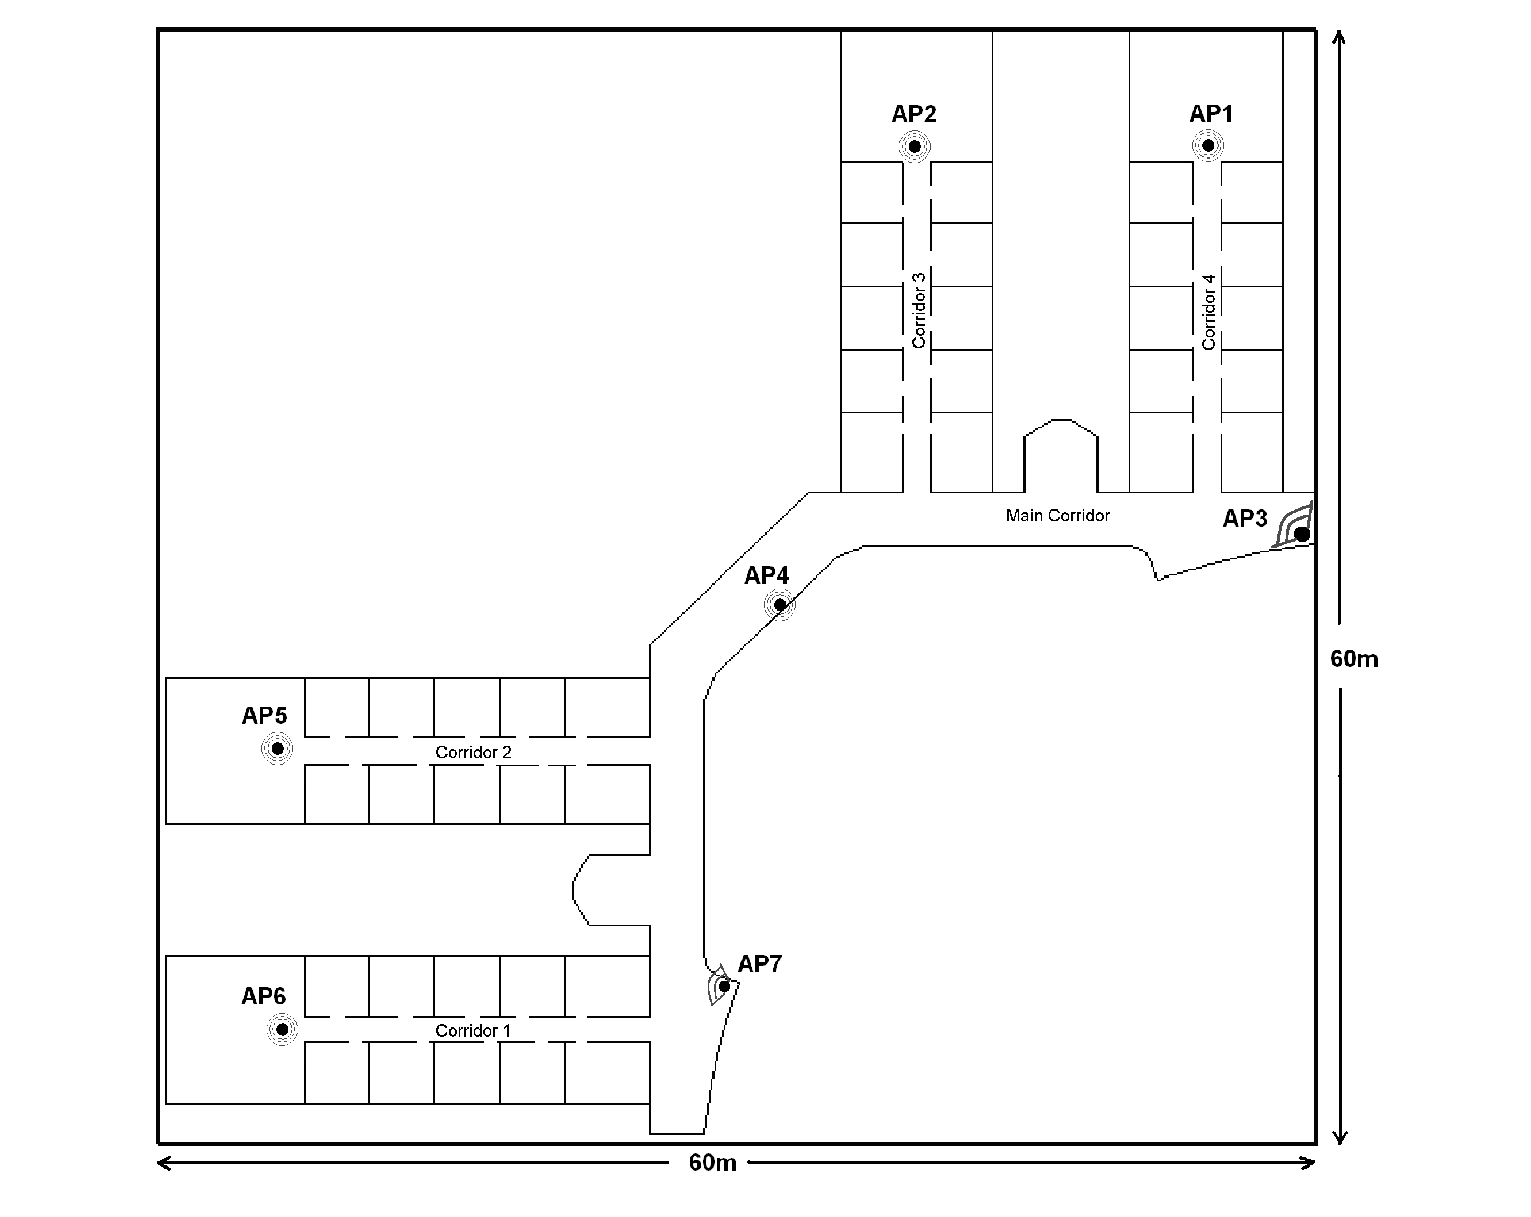
\includegraphics[width=4.7in]{Figure1}
  % where an .eps filename suffix will be assumed under latex, and a .pdf suffix will be assumed for pdflatex
  \caption{Departamento de Electrónica.}
  \label{fig:fig1}
\end{figure}

Y ahora un ejemplo en el que ponemos el \texttt{caption} en el lateral:

\begin{SCfigure}
  \centering 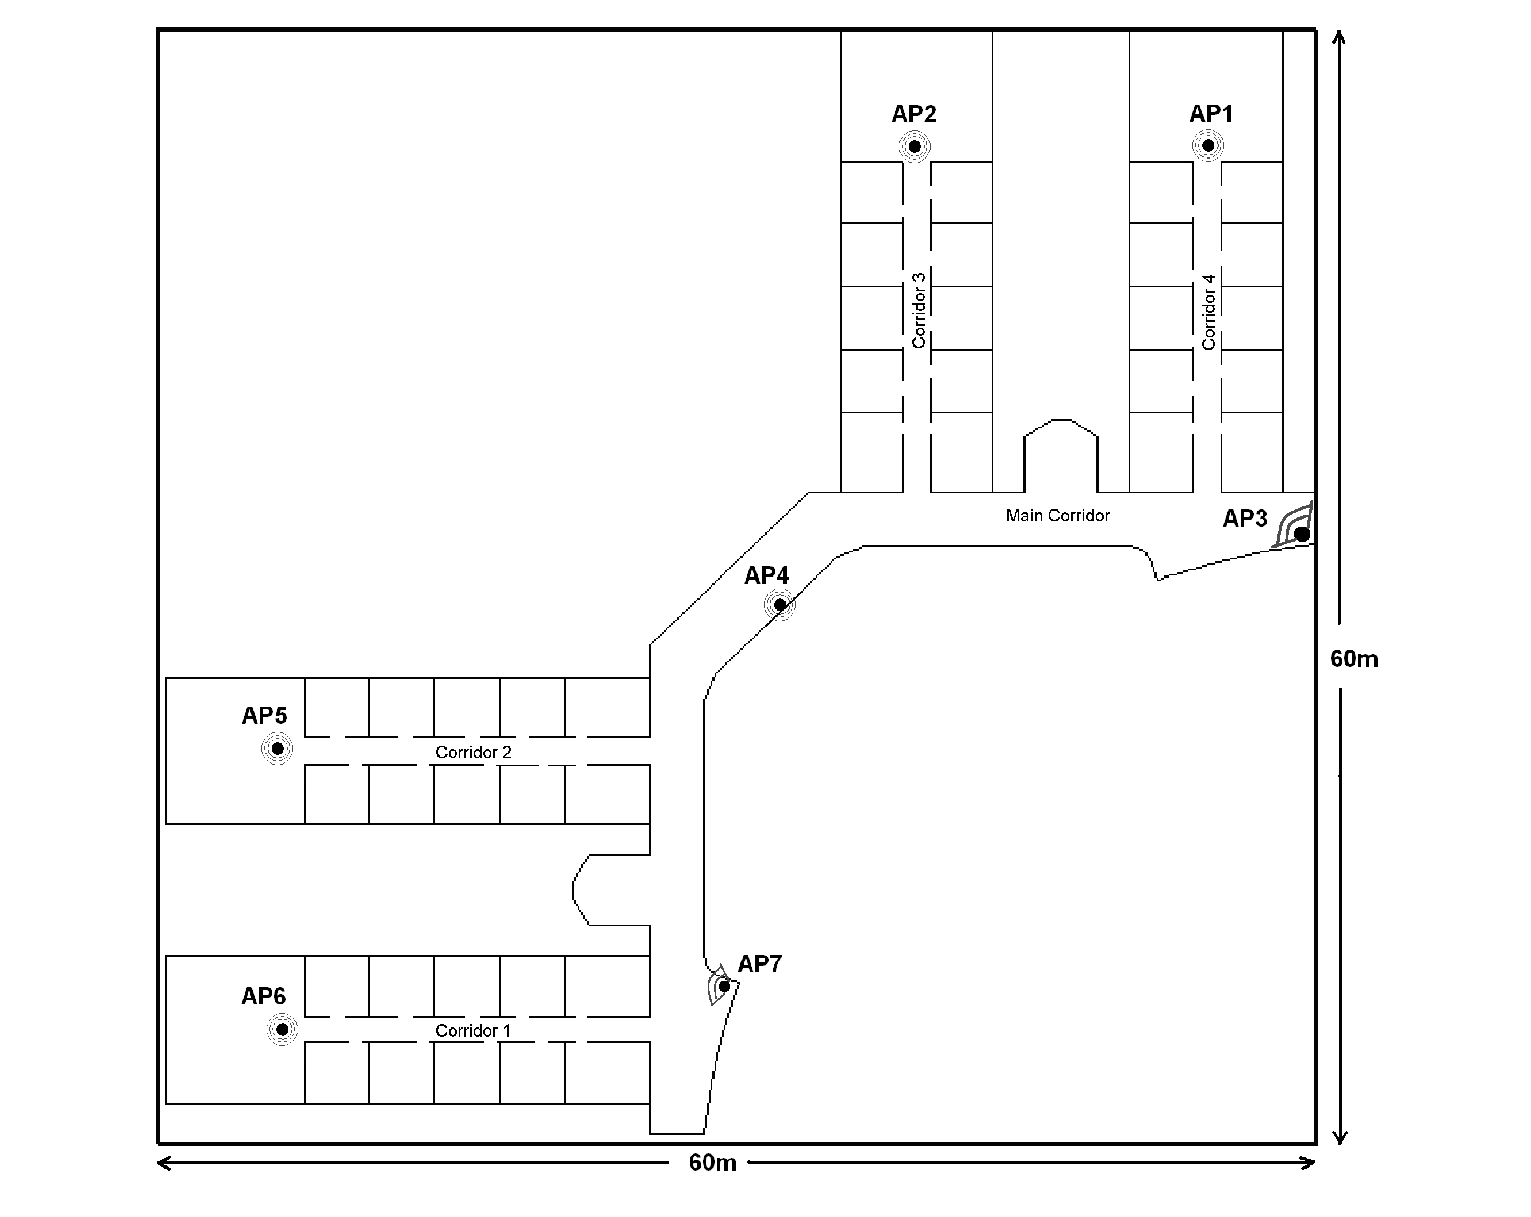
\includegraphics[width=0.5\textwidth]{Figure1}
  \caption{Departamento de Electrónica en el lateral.}
\end{SCfigure}



\section{Técnicas utilizadas}
\label{sec:tecnicas-utilizadas}

Aquí vamos a probar todos los niveles de sección disponibles, para evaluar la asignación de \texttt{tocdepth}...

Blah, blah, blah\ldots


\subsection{Subsección}
\label{sec:subseccion}


\subsubsection{Subsubsección}
\label{sec:subsubseccion}

\paragraph{Paragraph}
\label{sec:paragraph-1}


\subparagraph{Subparagraph}
\label{sec:subparagraph}



\section{Conclusiones}
\label{sec:conclusiones-teoria}

Blah, blah, blah\ldots

%%% Local Variables:
%%% TeX-master: "../book"
%%% End:


%%%%%%%%%%%%%%%%%%%%%%%%%%%%%%%%%%%%%%%%%%%%%%%%%%%%%%%%%%%%%%%%%%%%%%%%%%%
%
% Generic template for TFC/TFM/TFG/Tesis
%
% $Id: desarrollo.tex,v 1.1 2015/06/05 00:05:19 macias Exp $
%
% By:
%  + Javier Macías-Guarasa. 
%    Departamento de Electrónica
%    Universidad de Alcalá
%  + Roberto Barra-Chicote. 
%    Departamento de Ingeniería Electrónica
%    Universidad Politécnica de Madrid   
% 
% Based on original sources by Roberto Barra, Manuel Ocaña, Jesús Nuevo,
% Pedro Revenga, Fernando Herránz and Noelia Hernández. Thanks a lot to
% all of them, and to the many anonymous contributors found (thanks to
% google) that provided help in setting all this up.
%
% See also the additionalContributors.txt file to check the name of
% additional contributors to this work.
%
% If you think you can add pieces of relevant/useful examples,
% improvements, please contact us at (macias@depeca.uah.es)
%
% You can freely use this template and please contribute with
% comments or suggestions!!!
%
%%%%%%%%%%%%%%%%%%%%%%%%%%%%%%%%%%%%%%%%%%%%%%%%%%%%%%%%%%%%%%%%%%%%%%%%%%%

\chapter{Desarrollo}
\label{cha:development}


\begin{FraseCelebre}
  \begin{Frase}
    A fuerza de construir bien, se llega a buen
    arquitecto\footnote{Tomado de ejemplos del proyecto \texis{}.}.
  \end{Frase}
  \begin{Fuente}
    Aristóteles
  \end{Fuente}
\end{FraseCelebre}



\section{Introducción}
\label{sec:development-introduction}

Blah, blah, blah.

La estructura de este capítulo es\ldots


\section{Sección 1 del capítulo de desarrollo}
\label{sec:development-1}

Blah, blah, blah.


\subsection{Subsección 1.1 del capítulo de desarrollo}
\label{sec:development-11}

Blah, blah, blah.


\subsection{Subsección 1.2 del capítulo de desarrollo}
\label{sec:development-12}

Blah, blah, blah.



\section{Sección 2 del capítulo de desarrollo}
\label{sec:development-2}

Blah, blah, blah.




\section{Conclusiones}
\label{sec:development-conclusions}

Blah, blah, blah.



%%% Local Variables:
%%% TeX-master: "../book"
%%% End:


%%%%%%%%%%%%%%%%%%%%%%%%%%%%%%%%%%%%%%%%%%%%%%%%%%%%%%%%%%%%%%%%%%%%%%%%%%%
%
% Generic template for TFC/TFM/TFG/Tesis
%
% $Id: resultados.tex,v 1.7 2016/03/31 10:44:23 macias Exp $
%
% By:
%  + Javier Macías-Guarasa.
%    Departamento de Electrónica
%    Universidad de Alcalá
%  + Roberto Barra-Chicote.
%    Departamento de Ingeniería Electrónica
%    Universidad Politécnica de Madrid
% 
% Based on original sources by Roberto Barra, Manuel Ocaña, Jesús Nuevo, Pedro Revenga, Fernando Herránz and Noelia Hernández. Thanks a lot to all of them, and to the many anonymous contributors found (thanks to google) that provided help in setting all this up.
%
% See also the additionalContributors.txt file to check the name of additional contributors to this work.
%
% If you think you can add pieces of relevant/useful examples, improvements, please contact us at (macias@depeca.uah.es)
%
% You can freely use this template and please contribute with comments or suggestions!!!
%
%%%%%%%%%%%%%%%%%%%%%%%%%%%%%%%%%%%%%%%%%%%%%%%%%%%%%%%%%%%%%%%%%%%%%%%%%%%

\chapter{Resultados}
\label{cha:resultados}


\begin{FraseCelebre}
  \begin{Frase}
    % Si quieres ser leído más de una vez, no vaciles en borrar a menudo.
    Rem tene, verba sequentur (Si dominas el tema, las palabras vendrán solas)\footnote{Tomado de ejemplos del proyecto \texis{}.}.
  \end{Frase}
  \begin{Fuente}
    % Horacio
    Catón el Viejo
  \end{Fuente}
\end{FraseCelebre}

\section{Introducción}
\label{sec:introduccion-resultados}

En este capítulo se introducirán los resultados más relevantes del trabajo.

La estructura del capítulo es\ldots


\section{Entorno experimental}
\label{sec:entorno-experimental}

Blah, blah, blah.


\subsection{Bases de datos utilizadas}
\label{sec:bases-de-datos-1}

Blah, blah, blah.


\subsection{Métricas de calidad}
\label{sec:metricas-de-calidad}

Blah, blah, blah.

En la tabla\ref{pruebaCalc2LaTeX} pongo un ejemplo del uso del conversor de libreoffice a \LaTeX{} (cortesía de Roberto Chamorro). Para usarlo tienes que importar la macro que encontrarás en el directorio \texttt{Tools/calc2latex//calc2latex\_024\_eur\_latex}\footnote{Para ello sigue el proceso de importación que se describe en \url{http://ask.libreoffice.org/en/question/35598/where-are-lo-basic-macros-stored/}, importando Cals y cuando ejecutes la macro hazlo por el punto de entrada \texttt{Main}, después de seleccionar el rango de celdas de la tabla.}

\begin{table}[htbp]
\caption{Caption de prueba de tabla LaTeX convertida desde
  \texttt{libreoffice} con la macro \texttt{calc2latex}.}
\begin{center}
\begin{tabular}{|l|r|r|r|}
\hline
 & \multicolumn{1}{l|}{System A} & \multicolumn{1}{l|}{System B} & \multicolumn{1}{l|}{System C} \\ \hline
FA rate & 10,00\% & 5,00\% & 2,00\% \\ \hline
TA rate & 90,00\% & 85,00\% & 75,00\% \\ \hline
\end{tabular}
\end{center}
\label{pruebaCalc2LaTeX}
\end{table}




\subsection{Estrategia y metodología de experimentación}
\label{sec:estr-y-metod}

Blah, blah, blah.


\section{Resultados experimentales}
\label{sec:result-experim}

A continuación, se muestra un ejemplo de tabla simple (ver tabla \ref{tab:table1}).

\begin{table}
  % increase table row spacing, adjust to taste
  \renewcommand{\arraystretch}{1.3}
  \caption{Comparativa.}
  \label{tab:table1}
  \begin{center}
    % Some packages, such as MDW tools, offer better commands for making tables than the plain LaTeX2e tabular which is used here.
    \begin{tabular}{|c|c|c|}
      \hline
      Method & Training Time & Man-Work (\%)\\
      \hline
      Propagation model & $<$ 30 sec & 5\\
      \hline
      Manual & 9 h 30 min & 24\\
      \hline
      Automatic & 2 h & 10 8\\
      \hline
    \end{tabular}
  \end{center}
\end{table}

Cuando las tablas ocupan más de un página se debe utilizar un tipo especial de tablas denominado \texttt{longtable}. A continuación, se muestra un ejemplo del mismo (ver tabla \ref{table2}).

\begin{center}
	\begin{longtable}{|c|c|c|c|}
    \caption[Resultados de la correlación cruzada.]{Resultados de la correlación cruzada.} \label{table2} \\
    
    \hline \multicolumn{1}{|c|}{\textbf{Posición Real}} & \multicolumn{1}{c|}{\textbf{Posición estimada}} & \multicolumn{1}{c|}{\textbf{Coef. Correlación}} & \multicolumn{1}{c|}{\textbf{Acierto/Fallo}} \\ \hline 
    \endfirsthead
    
    \multicolumn{4}{c}%
    {{\bfseries \tablename\ \thetable{} -- continúa en la página anterior}} \\
    \hline \multicolumn{1}{|c|}{\textbf{Posición Real}} & \multicolumn{1}{c|}{\textbf{Posición estimada}} & \multicolumn{1}{c|}{\textbf{Coef. Correlación}} & \multicolumn{1}{c|}{\textbf{Acierto/Fallo}} \\ \hline 
    \endhead
    
    \hline \multicolumn{4}{|r|}{{Continúa en la página siguiente}} \\ \hline
    \endfoot

    \hline \hline
    \endlastfoot
    
    \hline	2P0	&	2P0	&	0,004954	&	A	\\
    \hline	2P1	&	2P4	&	0,005752	&	F	\\
    \hline	2P2	&	2P2	&	0,005461	&	A	\\
    \hline	2P3	&	2P0	&	0,004634	&	F	\\
    \hline	2P5	&	2P4	&	0,005991	&	F	\\
    \hline	2P6	&	2P16	&	0,004410	&	F	\\
    \hline	2P7	&	3P9	&	0,008038	&	F	\\
    \hline	2P8	&	3P9	&	0,003753	&	F	\\
    \hline	2P9	&	2P7	&	0,004908	&	F	\\
    \hline	2P10	&	2P10	&	0,007273	&	A	\\
    \hline	2P14	&	2P16	&	0,006485	&	F	\\
    \hline	2P15	&	2P15	&	0,004932	&	A	\\
    \hline	2P16	&	2P16	&	0,006237	&	A	\\
    \hline	2P17	&	2P15	&	0,005110	&	F	\\
    \hline	2P18	&	3P18	&	0,006235	&	F	\\
    \hline	2P19	&	3P18	&	0,004827	&	F	\\
    \hline	2P20	&	2P20	&	0,006877	&	A	\\
    \hline	2P22	&	3P18	&	0,003048	&	F	\\
    \hline	2P24	&	2P24	&	0,006833	&	A	\\
    \hline	2P25	&	2P25	&	0,004875	&	A	\\
    \hline	2P26	&	2P31	&	0,005511	&	F	\\
    \hline	2P27	&	2P28	&	0,004590	&	F	\\
    \hline	2P30	&	2P31	&	0,005576	&	F	\\
    \hline	2P31	&	2P31	&	0,007213	&	A	\\
    \hline	2P32	&	2P35	&	0,003340	&	F	\\
    \hline	2P34	&	2P34	&	0,004128	&	A	\\
    \hline	2P36	&	2P35	&	0,003329	&	F	\\
    \hline	2P37	&	2P37	&	0,003468	&	A	\\
    \hline	2P39	&	2P38	&	0,002577	&	F	\\
    \hline	2P40	&	2P43	&	0,004303	&	F	\\
    \hline	2P41	&	2P41	&	0,001573	&	A	\\
    \hline	2P42	&	2P41	&	0,000846	&	F	\\
    \hline	2P44	&	2P44	&	0,002732	&	A	\\
    \hline	2P45	&	23P45	&	0,001958	&	F	\\
    \hline	2P47	&	2P34	&	0,002869	&	F	\\
    \hline	2P48	&	2P43	&	0,004569	&	F	\\
    \hline	2P49	&	3P51	&	0,001374	&	F	\\
    \hline	2P50	&	2P34	&	0,002274	&	F	\\
    \hline	2P51	&	2P63	&	0,003931	&	F	\\
    \hline	2P52	&	2P55	&	0,003537	&	F	\\
    \hline	2P53	&	3P56	&	0,003126	&	F	\\
    \hline	2P54	&	2P67	&	0,005560	&	F	\\
    \hline	2P56	&	2P55	&	0,002817	&	F	\\
    \hline	2P57	&	2P67	&	0,006168	&	F	\\
    \hline	2P58	&	2P58	&	0,005278	&	A	\\
    \hline	2P60	&	3P66	&	0,004966	&	F	\\
    \hline	2P61	&	3P61	&	0,004748	&	A	\\
    \hline	2P64	&	2P67	&	0,005342	&	F	\\
    \hline	2P66	&	2P4	&	0,004172	&	F	\\
    \hline	2P67	&	2P67	&	0,005706	&	A	\\
    \hline	3P0	&	3P0	&	0,003674	&	A	\\
    \hline	3P61	&	2P61	&	0,003263	&	F	\\
    \hline	3P64	&	2P67	&	0,003484	&	F	\\
    \hline	3P65	&	2P67	&	0,002975	&	F	\\
    \hline	3P66	&	2P58	&	0,005029	&	F	\\
    \hline	3P67	&	3P67	&	0,003714	&	A	\\
	\end{longtable}
\end{center}

En algunas ocasiones, también resulta útil emplear el entorno
\texttt{subfigure} para añadir múltiples imágenes dentro de la misma
figura. A continuación, se muestra un ejemplo del uso en la figura
\ref{fig:fig3}. También se pueden referenciar las sub-figuras de forma
individual, por ejemplo la sub-figura \ref{fig:fig3b} (usando un método
de cita), o bien la sub-figura \ref{fig:fig3}.\subref{fig:fig3b} (usando
otro alternativo).

% For this to work you need to (in preamble.tex):
% - remove \usepackage{subfig}
% - add \usepackage{caption}
% - add \usepackage{subcaption}
\begin{figure}
  \centering
  \begin{subfigure}[b]{0.3\textwidth}
    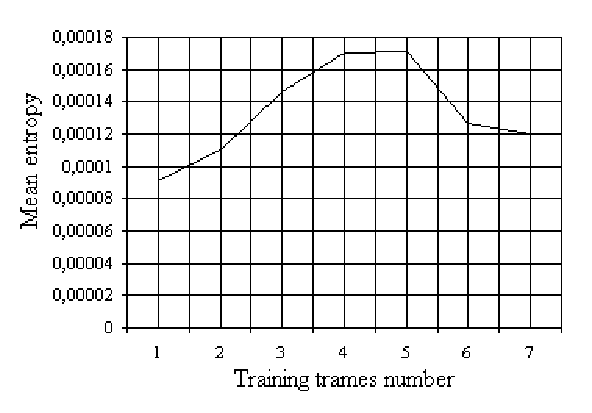
\includegraphics[width=\textwidth]{Figure2}
    \caption{Mean Entropy.}
    \label{fig:fig3a}
  \end{subfigure}%
  ~ %add desired spacing between images, e. g. ~, \quad, \qquad etc.
  % (or a blank line to force the subfigure onto a new line)
  \begin{subfigure}[b]{0.3\textwidth}
    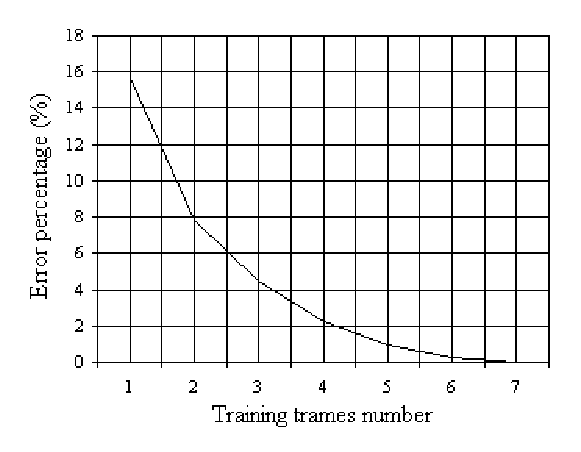
\includegraphics[width=\textwidth]{Figure3}
    \caption{Error Percentage.}
    \label{fig:fig3b}
  \end{subfigure}
  \caption{Optimal trames number in the training data set.}
  \label{fig:fig3}
\end{figure}

La figura~\ref{fig:LIdiapRoom} muestra otro ejemplo con referencias a las subfigures en el caption principal.

\begin{figure}
  \centering
  \begin{subfigure}[b]{0.30\textwidth}
    
\includegraphics[width=\textwidth]{roomlayout2}
    \caption{}
    \label{fig:RoomLayout}
  \end{subfigure}%
  \qquad \qquad %add desired spacing between images, e. g. ~, \quad, \qquad, \hfill etc.
  % (or a blank line to force the subfigure onto a new line)
  \begin{subfigure}[b]{0.425\textwidth}
    \includegraphics[width=\textwidth]{idiap-seq45-cam2.jpg}
    \caption{}
    \label{fig:RoomPicture}
  \end{subfigure}
  \caption{Idiap Smart Meeting Room for AV16.3 recordings. (\protect\subref{fig:RoomLayout}) Room layout showing the centered table, and the microphones arranged in two circular arrays. (\protect\subref{fig:RoomPicture}) Sample of recorded video frame showing the arrays area. \vspace{-0.3cm}}
  \label{fig:LIdiapRoom}
\end{figure}

Os incluimos a continuación un párrafo de un artículo en el que hacemos referencia a varias figuras y subfiguras:

\emph{The IDIAP Meeting Room (shown in figure~\ref{fig:LIdiapRoom}) is a $8.2m \times 3.6m \times 2.4m$ rectangular space containing a centrally located $4.8m \times 1.2m$ rectangular table, on top of which two circular microphone arrays of $10 cm$ radius are located, each of them composed by 8 microphones. The centers of the two arrays are separated by $80 cm$ and the origin of coordinates is located in the middle point between the two arrays. The arrays can be also seen in figures~\ref{fig:simureal_positions}.\subref{fig:Simulated_positions}, ~\ref{fig:simureal_positions}.\subref{fig:real_positions_short}, and ~\ref{fig:simureal_positions}.\subref{fig:real_positions_long}, in which only the relevant section of the room is displayed, each one showing different scenarios that were used in the experiments. A detailed description of the meeting room can be found in~\cite{moore2002}.}

\begin{figure}
  \centering
  \begin{subfigure}[t]{0.3\textwidth}
    
\includegraphics[width=\textwidth]{angular2-short-improved}
    \caption{For validation\\with simulated data.}
    \label{fig:Simulated_positions}
  \end{subfigure}
~%add desired spacing between images, e. g. ~, \quad, \qquad,
  % \hfill etc.
  % (or a blank line to force the subfigure onto a new line)
  \begin{subfigure}[t]{0.3\textwidth}
    
\includegraphics[width=\textwidth]{positions1-short-improved}
    \caption{For validation\\with real data and microphone pairs with $20~cm$ spacing.}
    \label{fig:real_positions_short}
  \end{subfigure}
  ~
  \begin{subfigure}[t]{0.3\textwidth}
    
\includegraphics[width=\textwidth]{positions2-short-improved}
    \caption{For validation\\with real data and microphone pairs with
      $82.46~cm$ spacing.}
    \label{fig:real_positions_long}
  \end{subfigure}
  \caption{Geometrical details for the experiments carried out. Only the
    relevant section of the room is shown, and microphone pairs are
    connected by solid lines.}
  \label{fig:simureal_positions}
\end{figure}

En la figura~\ref{fig:Sim_angles} mostramos un ejemplo de varias
figuras organizadas de forma un poco más complejo.

\begin{figure}
  \centering
  \begin{subfigure}[b]{0.3\textwidth}
    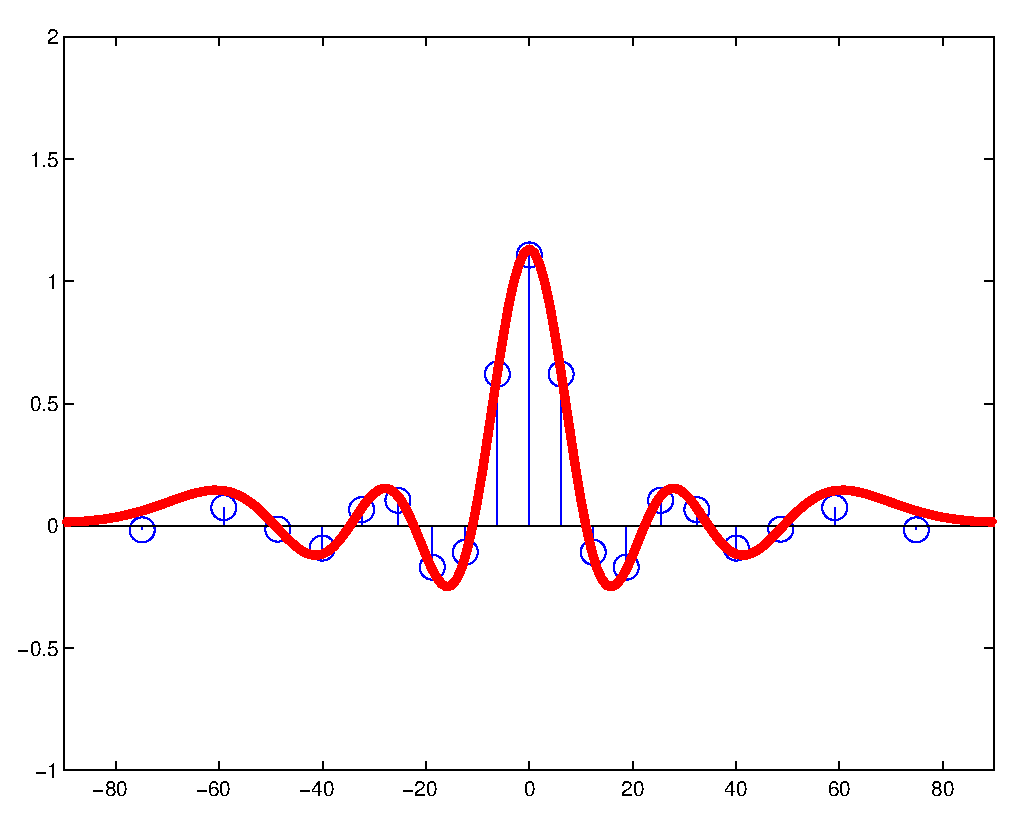
\includegraphics[width=\textwidth]{Sim_seg025_ang090}
    \caption{$0^{\circ}$}
    \label{fig:Sim_ang090}
  \end{subfigure}
  % add desired spacing between images, e. g. ~, \quad, \qquad etc.
  % (or a blank line to force the subfigure onto a new line)

  \begin{subfigure}[b]{0.3\textwidth}
    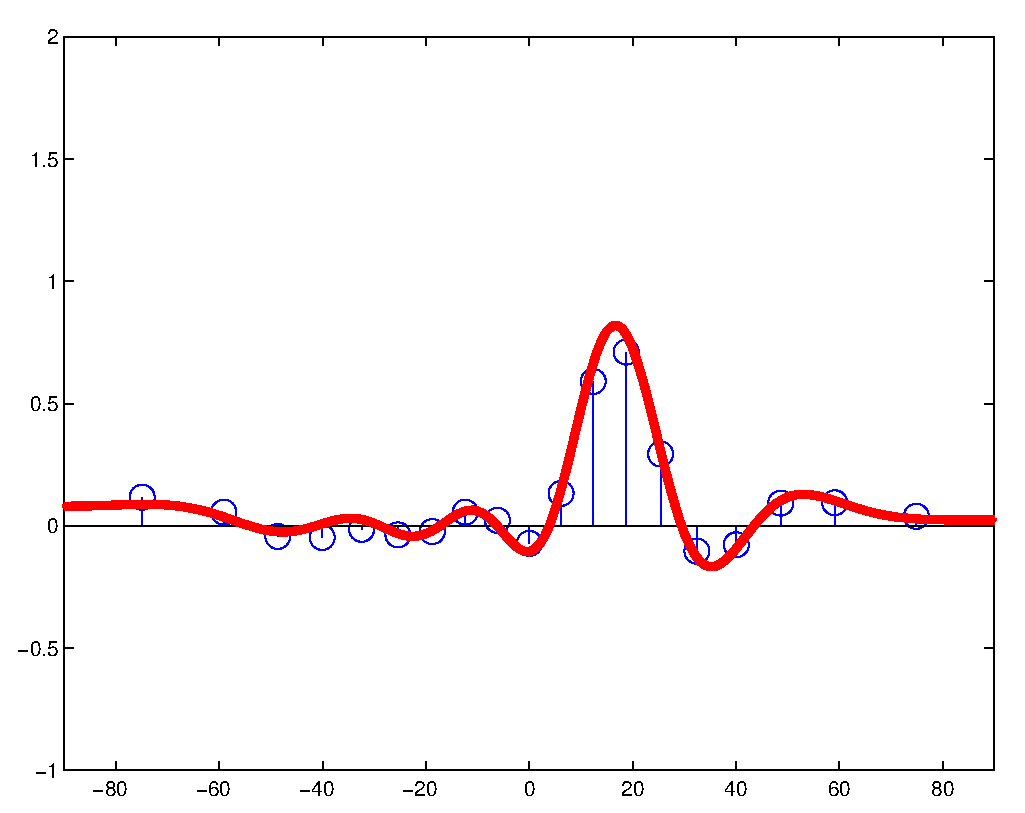
\includegraphics[width=\textwidth]{Sim_seg025_ang108}
    \caption{$18^{\circ}$}
    \label{fig:Sim_ang108}
  \end{subfigure}
  % add desired spacing between images, e. g. ~, \quad, \qquad etc.
  % (or a blank line to force the subfigure onto a new line)
  \begin{subfigure}[b]{0.3\textwidth}
    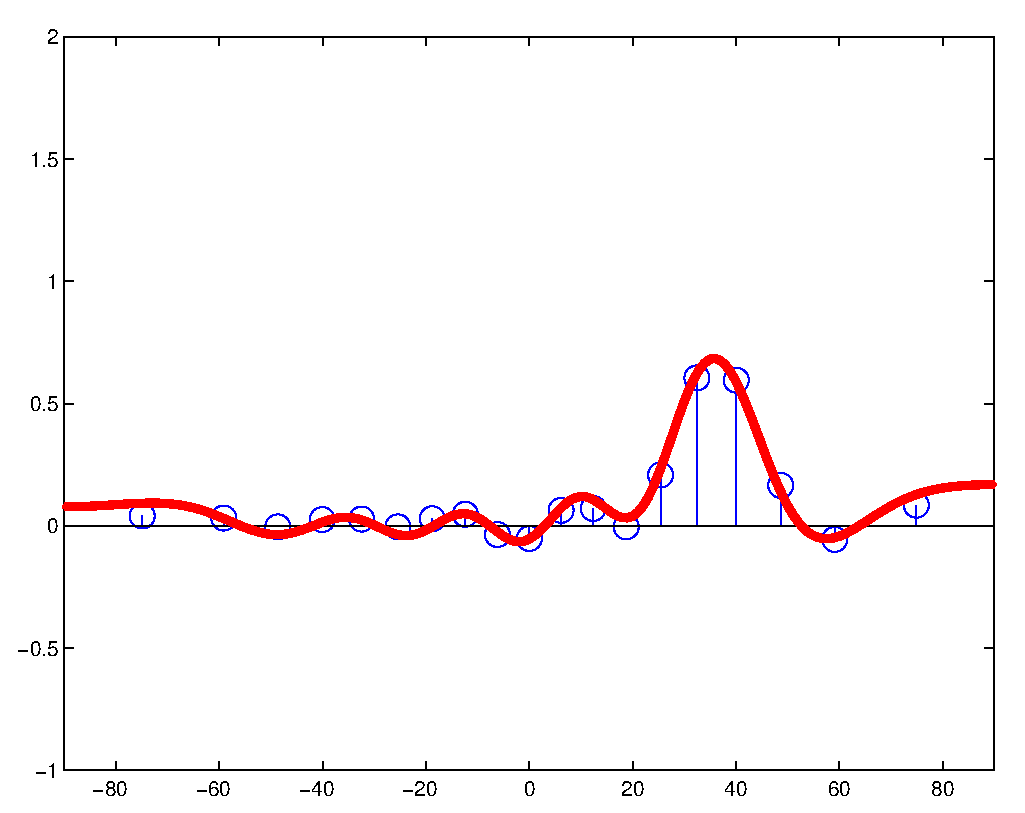
\includegraphics[width=\textwidth]{Sim_seg025_ang126}
    \caption{$36^{\circ}$}
    \label{fig:Sim_ang126}
  \end{subfigure}
  % add desired spacing between images, e. g. ~, \quad, \qquad etc.
  % (or a blank line to force the subfigure onto a new line)
  \begin{subfigure}[b]{0.3\textwidth}
    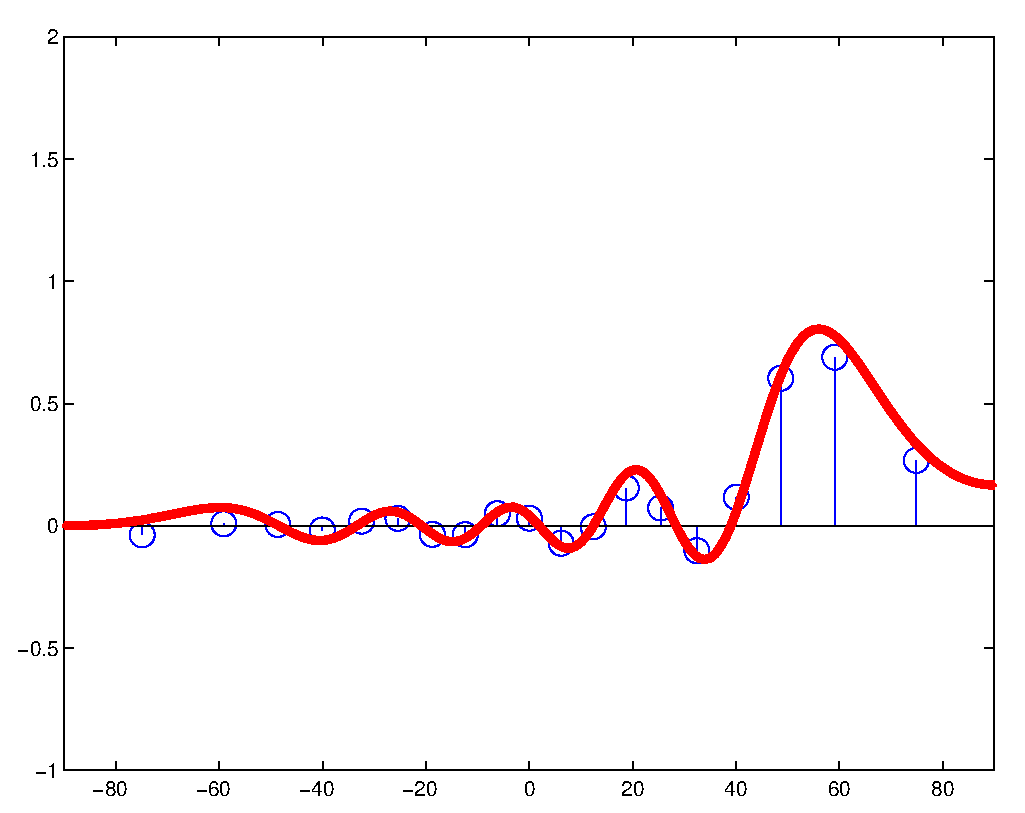
\includegraphics[width=\textwidth]{Sim_seg025_ang144}
    \caption{$54^{\circ}$}
    \label{fig:Sim_ang144}
  \end{subfigure}
  % add desired spacing between images, e. g. ~, \quad, \qquad etc.
  % (or a blank line to force the subfigure onto a new line)

  \begin{subfigure}[b]{0.3\textwidth}
    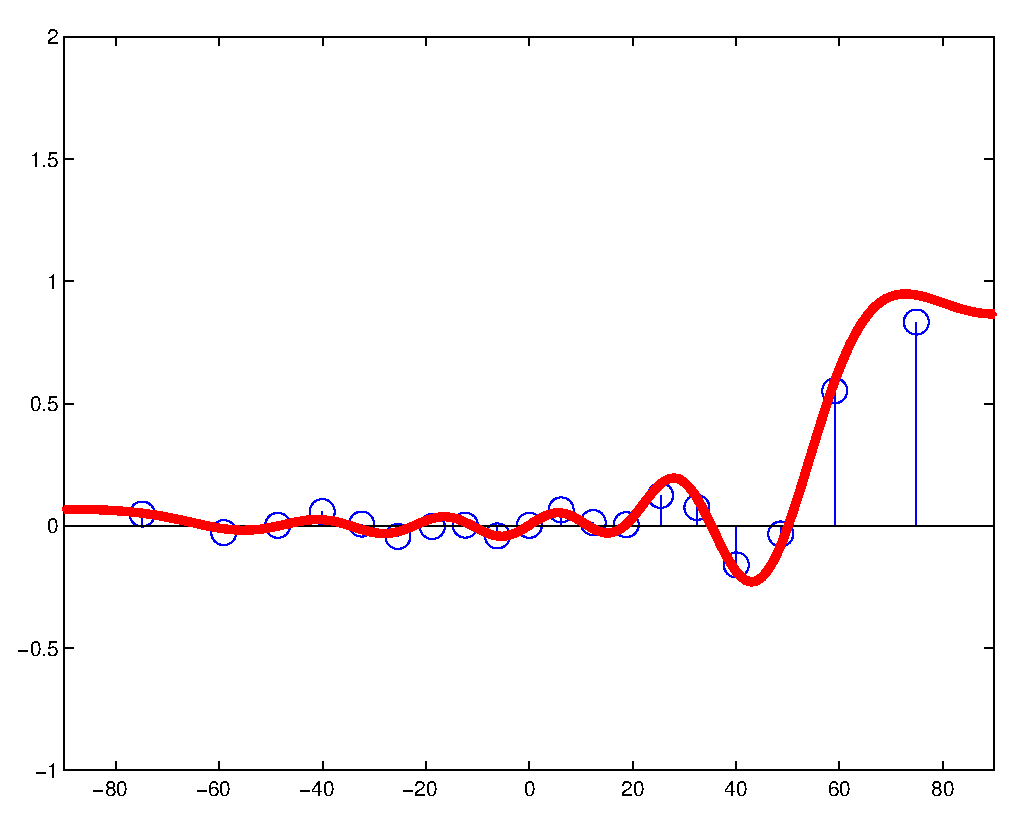
\includegraphics[width=\textwidth]{Sim_seg025_ang162}
    \caption{$72^{\circ}$}
    \label{fig:Sim_ang162}
  \end{subfigure}

  \caption{Comparison between the steered power response generated by the model (solid line) and that calculated using simulated waveforms in the AV16.3 environment (stems). Results for the speaker in given angles and the array steered from -90º to +90º are shown.}
  \label{fig:Sim_angles}
\end{figure}

También es posible incluir el código de una figura en un fichero \texttt{.tex} independiente (para hacer más legible el código del documento principal). Un ejemplo lo tenéis a continuación, incluyendo el texto en inglés del documento original:

\emph{Figure~\ref{fig:SRPvsPatternSelected} includes the results of the comparison, for several speaker positions (1, 2, 4, 6, 8 and 16, emphasized in figure~\ref{fig:simureal_positions}.\subref{fig:real_positions_short}), and selected to provide different acoustic situations, both in terms of distance and angular position with respect to the arrays. All the graphics show the acoustic power map (predicted or calculated) for a regular two-dimensional grid of $10~cm$. The plot is provided from a top view of the room, spanning the full plan at a height of $61~cm$ above the microphone arrays (this height was the ground truth one for sequence 01). For each speaker position shown, three graphics are plotted:}

\begin{itemize}
  \item \emph{The graphics on the left show the SRP-PHAT acoustic power maps generated by the proposed model (for example, the left graphic in figure~\ref{fig:SRPvsPatternSelected}.\subref{fig:SRPvsModel_Fo1500_position1} for position 1).}
  \item \emph{The graphics in the middle show the real SRP-PHAT acoustic power maps calculated using the real acoustic waveforms (for example, the middle graphic in figure~\ref{fig:SRPvsPatternSelected}.\subref{fig:SRPvsModel_Fo1500_position1} for position 1), for a single selected frame.}
  \item \emph{The graphics on the right show the average real SRP-PHAT acoustic power maps, averaging for all the frames in which the user was in the given position (for example, the right graphic in figure~\ref{fig:SRPvsPatternSelected}.\subref{fig:SRPvsModel_Fo1500_position1} for position 1).}
\end{itemize}

\emph{The green point represents the real (ground truth) speaker position, and the black dots represent the positions of the four microphones used. The hyperbolic shapes found in the figure are consistent with the fact that the place of points with equal acoustic power value, for a given microphone pair, is a hyperbola (in our two-dimensional case, being a hyperboloid of revolution in the three-dimensional case).}

\emph{From figure~\ref{fig:SRPvsPatternSelected}, it can clearly be seen that, again, the predictions closely match the results with real data for the different acoustic conditions, even when the simulations are using fixed and frequency independent average reflection coefficients, and that the acoustic model is based on the simplistic image method model.}

\begin{figure}
  \centering
  \begin{subfigure}[t]{0.47\textwidth}
    \begin{minipage}[t]{\textwidth}
      \begin{subfigure}[t]{0.3\textwidth}
        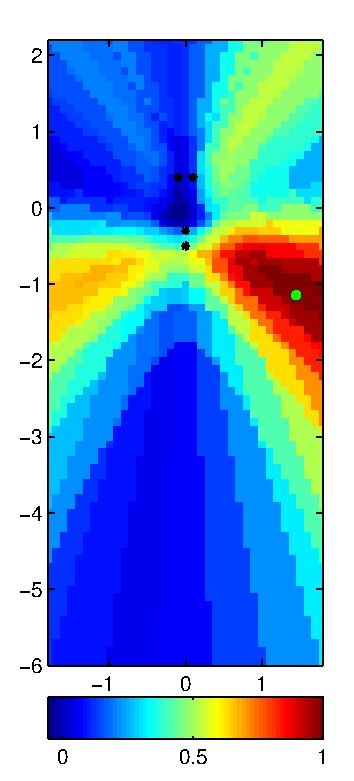
\includegraphics[width=\textwidth]{Pattern_Fo1500_pos01}
        %\caption{SRP Model for pos. 1}
        \label{fig:Pattern_Fo1500_pos01}
      \end{subfigure}
      % ~ %add desired spacing between images, e. g. ~, \quad, \qquad,
      % \hfill etc.
      % (or a blank line to force the subfigure onto a new line)
      \begin{subfigure}[t]{0.3\textwidth}
        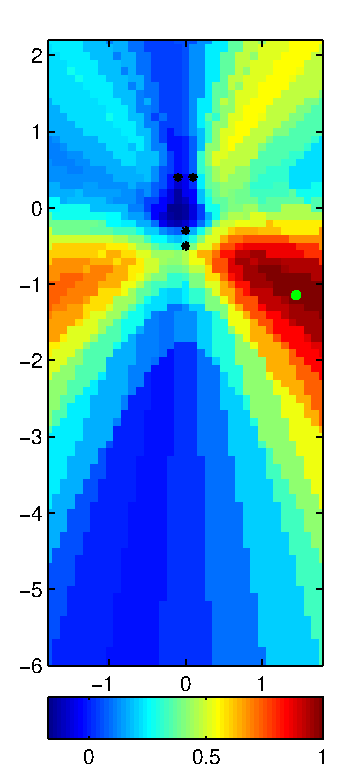
\includegraphics[width=\textwidth]{SRP_Fo1500_frame003_pos01}
        % \caption{Real SRP for pos.  1}
        \label{fig:SRP_Fo1500_pos01}
      \end{subfigure}
      % ~ %add desired spacing between images, e. g. ~, \quad, \qquad,
      % \hfill etc.
      % (or a blank line to force the subfigure onto a new line)
      \begin{subfigure}[t]{0.3\textwidth}
        \includegraphics[width=\textwidth]{SRP_Fo1500_mean_pos01}
        % \caption{Avg. SRP for pos. 1}
        \label{fig:SRP_Fo1500_mean_pos01}
      \end{subfigure}
      \vspace{\verticalSpacingSRPMaps}
      \caption{\centering For position 1}
      \label{fig:SRPvsModel_Fo1500_position1}
      \vspace{0.25cm}
    \end{minipage}
  \end{subfigure}
  ~% \quad % between 1 and 2 %add desired spacing between images, e. g. ~, \quad, \qquad,
  % \hfill etc.
  % (or a blank line to force the subfigure onto a new line)
  \begin{subfigure}[t]{0.47\textwidth}
    \begin{minipage}[t]{\textwidth}
      \begin{subfigure}[t]{0.3\textwidth}
        \includegraphics[width=\textwidth]{Pattern_Fo1500_pos02}
        % \caption{SRP Model for pos. 2}
        \label{fig:Pattern_Fo1500_pos02}
      \end{subfigure}
      % ~ %add desired spacing between images, e. g. ~, \quad, \qquad,
      % \hfill etc.
      % (or a blank line to force the subfigure onto a new line)
      \begin{subfigure}[t]{0.3\textwidth}
        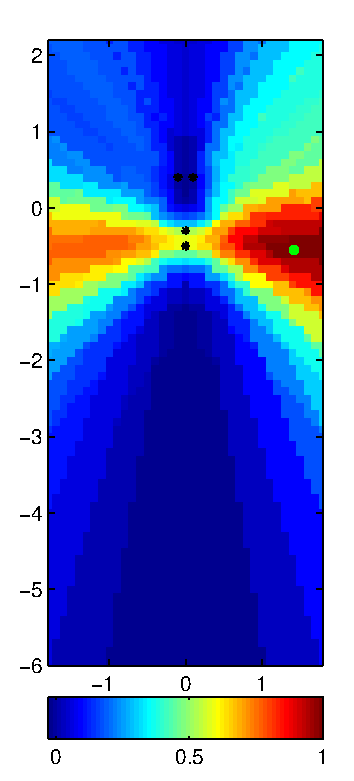
\includegraphics[width=\textwidth]{SRP_Fo1500_frame161_pos02}
        % \caption{Real SRP for pos.  2\\}
        \label{fig:SRP_pos02}
      \end{subfigure}
      % ~ %add desired spacing between images, e. g. ~, \quad, \qquad,
      % \hfill etc.
      % (or a blank line to force the subfigure onto a new line)
      \begin{subfigure}[t]{0.3\textwidth}
        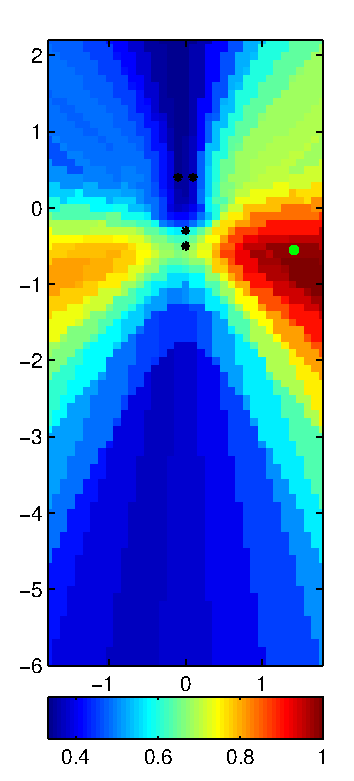
\includegraphics[width=\textwidth]{SRP_Fo1500_mean_pos02}
        % \caption{Avg. SRP for pos. 2}
        \label{fig:SRP_Fo1500_mean_pos02}
      \end{subfigure}
      \vspace{\verticalSpacingSRPMaps}
      \caption{\centering For position 2}
      \vspace{0.25cm}
    \end{minipage}
  \end{subfigure}

  \begin{subfigure}[t]{0.47\textwidth}
    \begin{minipage}[t]{\textwidth}
      \begin{subfigure}[t]{0.3\textwidth}
        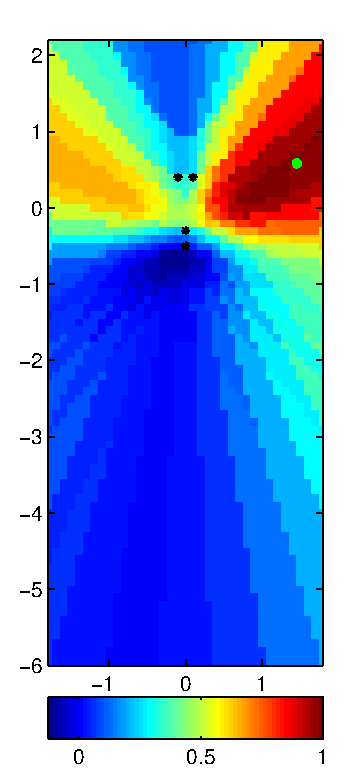
\includegraphics[width=\textwidth]{Pattern_Fo1500_pos04}
        % \caption{SRP Model for pos. 4}
        \label{fig:Pattern_Fo1500_pos04}
      \end{subfigure}
      % ~ %add desired spacing between images, e. g. ~, \quad, \qquad,
      % \hfill etc.
      % (or a blank line to force the subfigure onto a new line)
      \begin{subfigure}[t]{0.3\textwidth}
        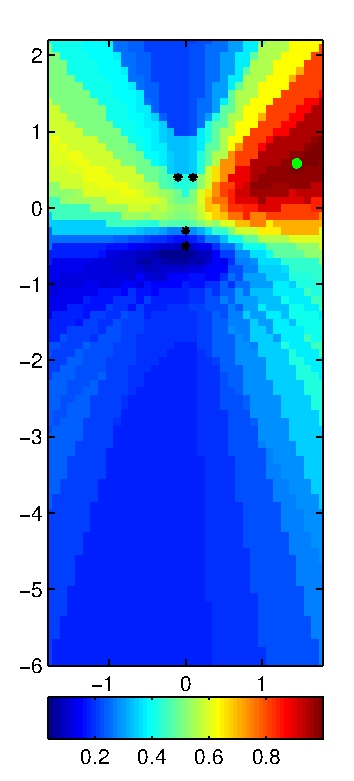
\includegraphics[width=\textwidth]{SRP_Fo1500_frame464_pos04}
        % \caption{Real SRP for pos.  4\\}
        \label{fig:SRP_pos04}
      \end{subfigure}
      % ~ %add desired spacing between images, e. g. ~, \quad, \qquad,
      % \hfill etc.
      % (or a blank line to force the subfigure onto a new line)
      \begin{subfigure}[t]{0.3\textwidth}
        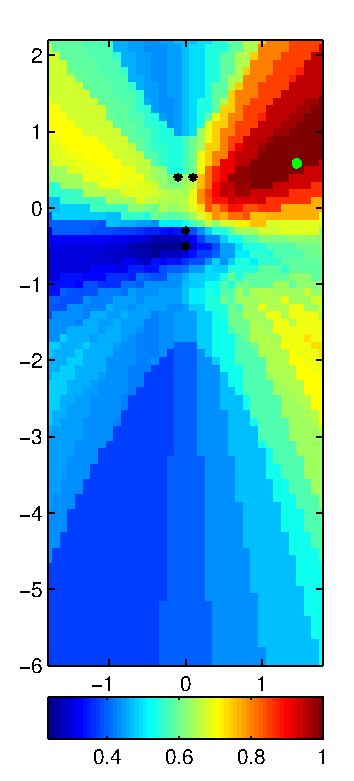
\includegraphics[width=\textwidth]{SRP_Fo1500_mean_pos04}
        % \caption{Avg. SRP for pos. 4}
        \label{fig:SRP_Fo1500_mean_pos04}
      \end{subfigure}
      \vspace{\verticalSpacingSRPMaps}
      \caption{\centering For position 4}
      \vspace{0.25cm}
    \end{minipage}
  \end{subfigure}
  ~%  \qquad % between 4 and 6 %add desired spacing between images, e. g. ~, \quad, \qquad,
  % \hfill etc.
  % (or a blank line to force the subfigure onto a new line)
  \begin{subfigure}[t]{0.47\textwidth}
    \begin{minipage}[t]{\textwidth}
      \begin{subfigure}[t]{0.3\textwidth}
        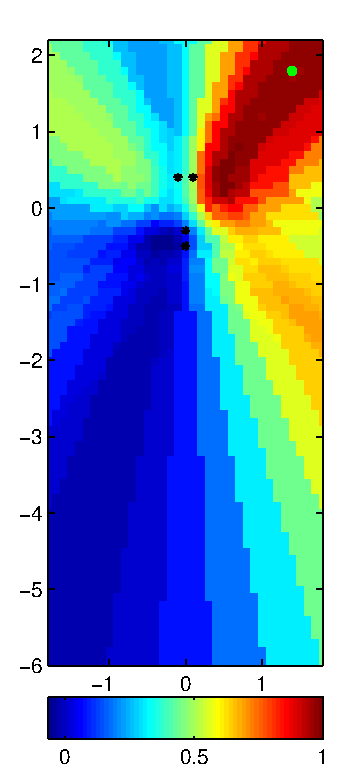
\includegraphics[width=\textwidth]{Pattern_Fo1500_pos06}
        % \caption{SRP Model for pos. 6}
        \label{fig:Pattern_Fo1500_pos06}
      \end{subfigure}
      % ~ %add desired spacing between images, e. g. ~, \quad, \qquad,
      % \hfill etc.
      % (or a blank line to force the subfigure onto a new line)
      \begin{subfigure}[t]{0.3\textwidth}
        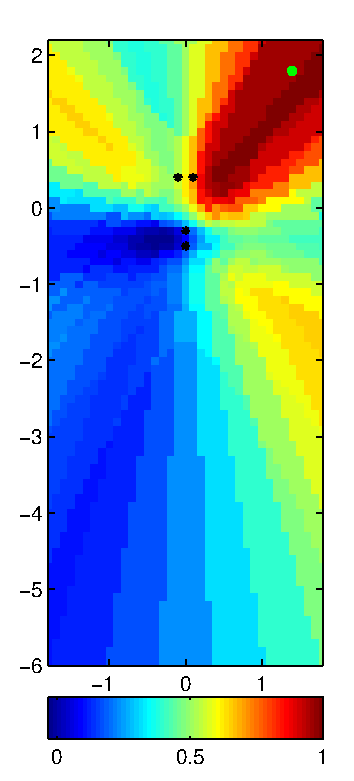
\includegraphics[width=\textwidth]{SRP_Fo1500_frame809_pos06}
        % \caption{Real SRP for pos.  6\\}
        \label{fig:SRP_pos06}
      \end{subfigure}
      % ~ %add desired spacing between images, e. g. ~, \quad, \qquad,
      % \hfill etc.
      % (or a blank line to force the subfigure onto a new line)
      \begin{subfigure}[t]{0.3\textwidth}
        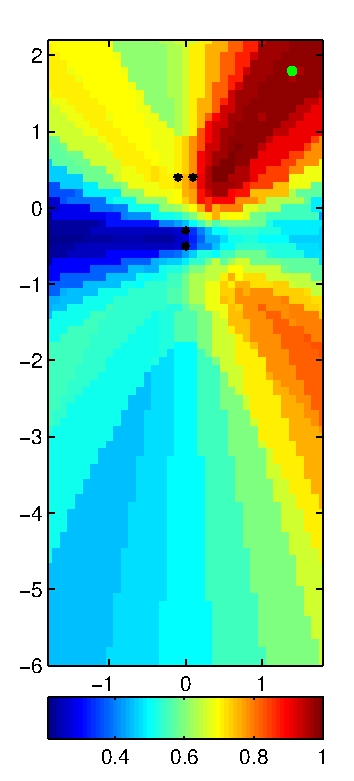
\includegraphics[width=\textwidth]{SRP_Fo1500_mean_pos06}
        % \caption{Avg. SRP for pos. 6}
        \label{fig:SRP_Fo1500_mean_pos06}
      \end{subfigure}
      \vspace{\verticalSpacingSRPMaps}
      \caption{\centering For position 6}
      \vspace{0.25cm}
    \end{minipage}
  \end{subfigure}

  \begin{subfigure}[t]{0.47\textwidth}
    \begin{minipage}[t]{\textwidth}
      \begin{subfigure}[t]{0.3\textwidth}
        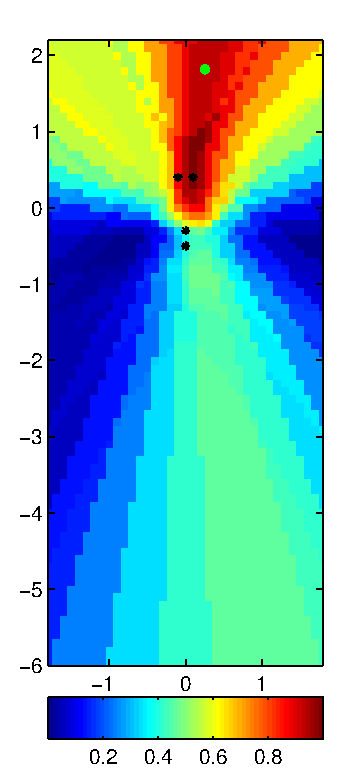
\includegraphics[width=\textwidth]{Pattern_Fo1500_pos08}
        % \caption{SRP Model for pos. 8}
        \label{fig:Pattern_Fo1500_pos08}
      \end{subfigure}
      % ~ %add desired spacing between images, e. g. ~, \quad, \qquad,
      % \hfill etc.
      % (or a blank line to force the subfigure onto a new line)
      \begin{subfigure}[t]{0.3\textwidth}
        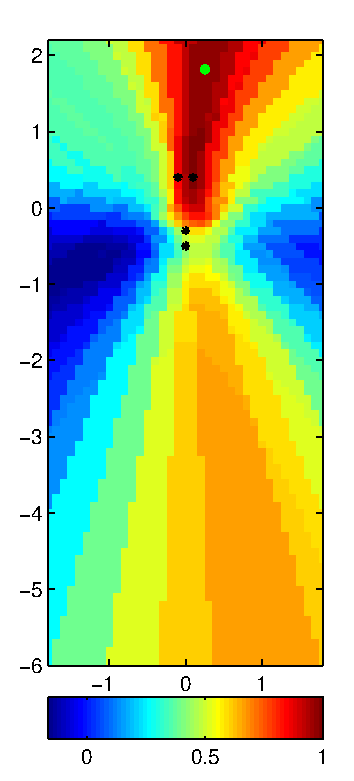
\includegraphics[width=\textwidth]{SRP_Fo1500_frame1127_pos08}
        % \caption{Real SRP for pos.  8\\}
        \label{fig:SRP_pos08}
      \end{subfigure}
      % ~ %add desired spacing between images, e. g. ~, \quad, \qquad,
      % \hfill etc.
      % (or a blank line to force the subfigure onto a new line)
      \begin{subfigure}[t]{0.3\textwidth}
        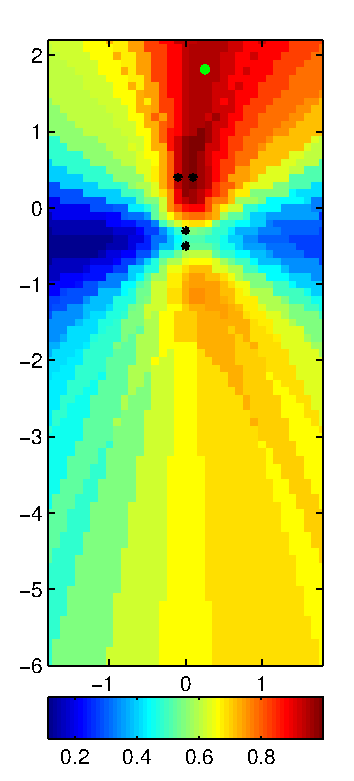
\includegraphics[width=\textwidth]{SRP_Fo1500_mean_pos08}
        % \caption{Avg. SRP for pos. 8}
        \label{fig:SRP_Fo1500_mean_pos08}
      \end{subfigure}
      \vspace{\verticalSpacingSRPMaps}
      \caption{\centering For position 8}
      \vspace{0.25cm}
    \end{minipage}
  \end{subfigure}
  ~%  \qquad % between 8 and 16 %add desired spacing between images, e. g. ~, \quad, \qquad,
  % \hfill etc.
  % (or a blank line to force the subfigure onto a new line)
  \begin{subfigure}[t]{0.47\textwidth}
    \begin{minipage}[t]{\textwidth}
      \begin{subfigure}[t]{0.3\textwidth}
        \includegraphics[width=\textwidth]{Pattern_Fo1500_pos16}
        % \caption{SRP Model for pos. 16}
        \label{fig:Pattern_Fo1500_pos16}
      \end{subfigure}
      % ~ %add desired spacing between images, e. g. ~, \quad, \qquad,
      % \hfill etc.
      % (or a blank line to force the subfigure onto a new line)
      \begin{subfigure}[t]{0.3\textwidth}
        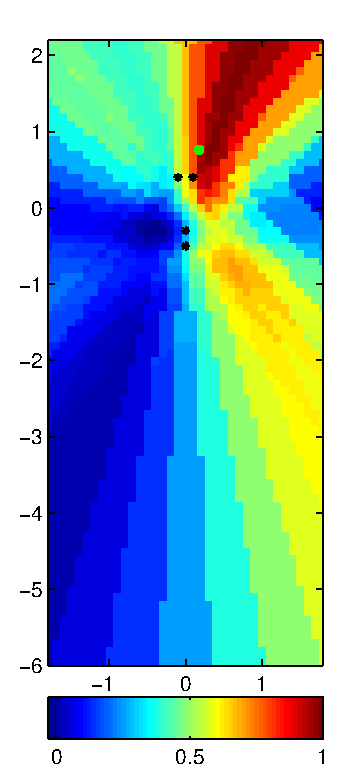
\includegraphics[width=\textwidth]{SRP_Fo1500_frame2518_pos16}
        % \caption{Real SRP for pos. 16\\}
        \label{fig:SRP_pos16}
      \end{subfigure}
      % ~ %add desired spacing between images, e. g. ~, \quad, \qquad,
      % \hfill etc.
      % (or a blank line to force the subfigure onto a new line)
      \begin{subfigure}[t]{0.3\textwidth}
        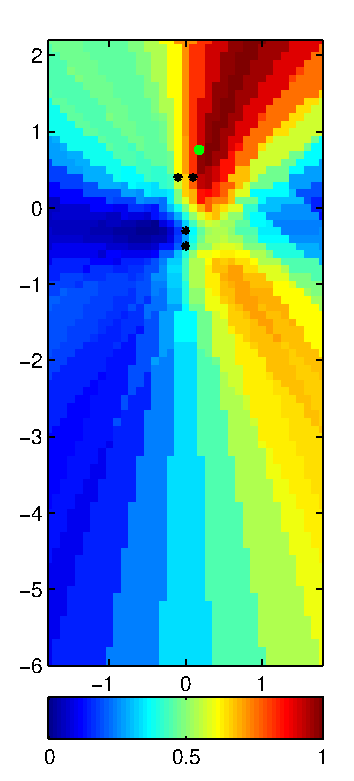
\includegraphics[width=\textwidth]{SRP_Fo1500_mean_pos16}
        % \caption{Avg. SRP for pos. 16}
        \label{fig:SRP_Fo1500_mean_pos16}
      \end{subfigure}
      \vspace{\verticalSpacingSRPMaps}
      \caption{\centering For position 16}
      \vspace{0.25cm}
    \end{minipage}
  \end{subfigure}
  \caption{Comparison between the SRP-PHAT map predicted by the model
    (left graphics),
    the real SRP-PHAT map (middle graphics), and the average (real)
    SRP-PHAT map (right graphics), for
    several speaker positions ($f_0=1.5~KHz$). See
    figure~~\ref{fig:simureal_positions}.\subref{fig:real_positions_short}
    for geometrical references.}
  \label{fig:SRPvsPatternSelected}
\end{figure}
 

\begin{wrapfigure}{r}{0.5\textwidth} 
\vspace{-20pt}
  \begin{center}
    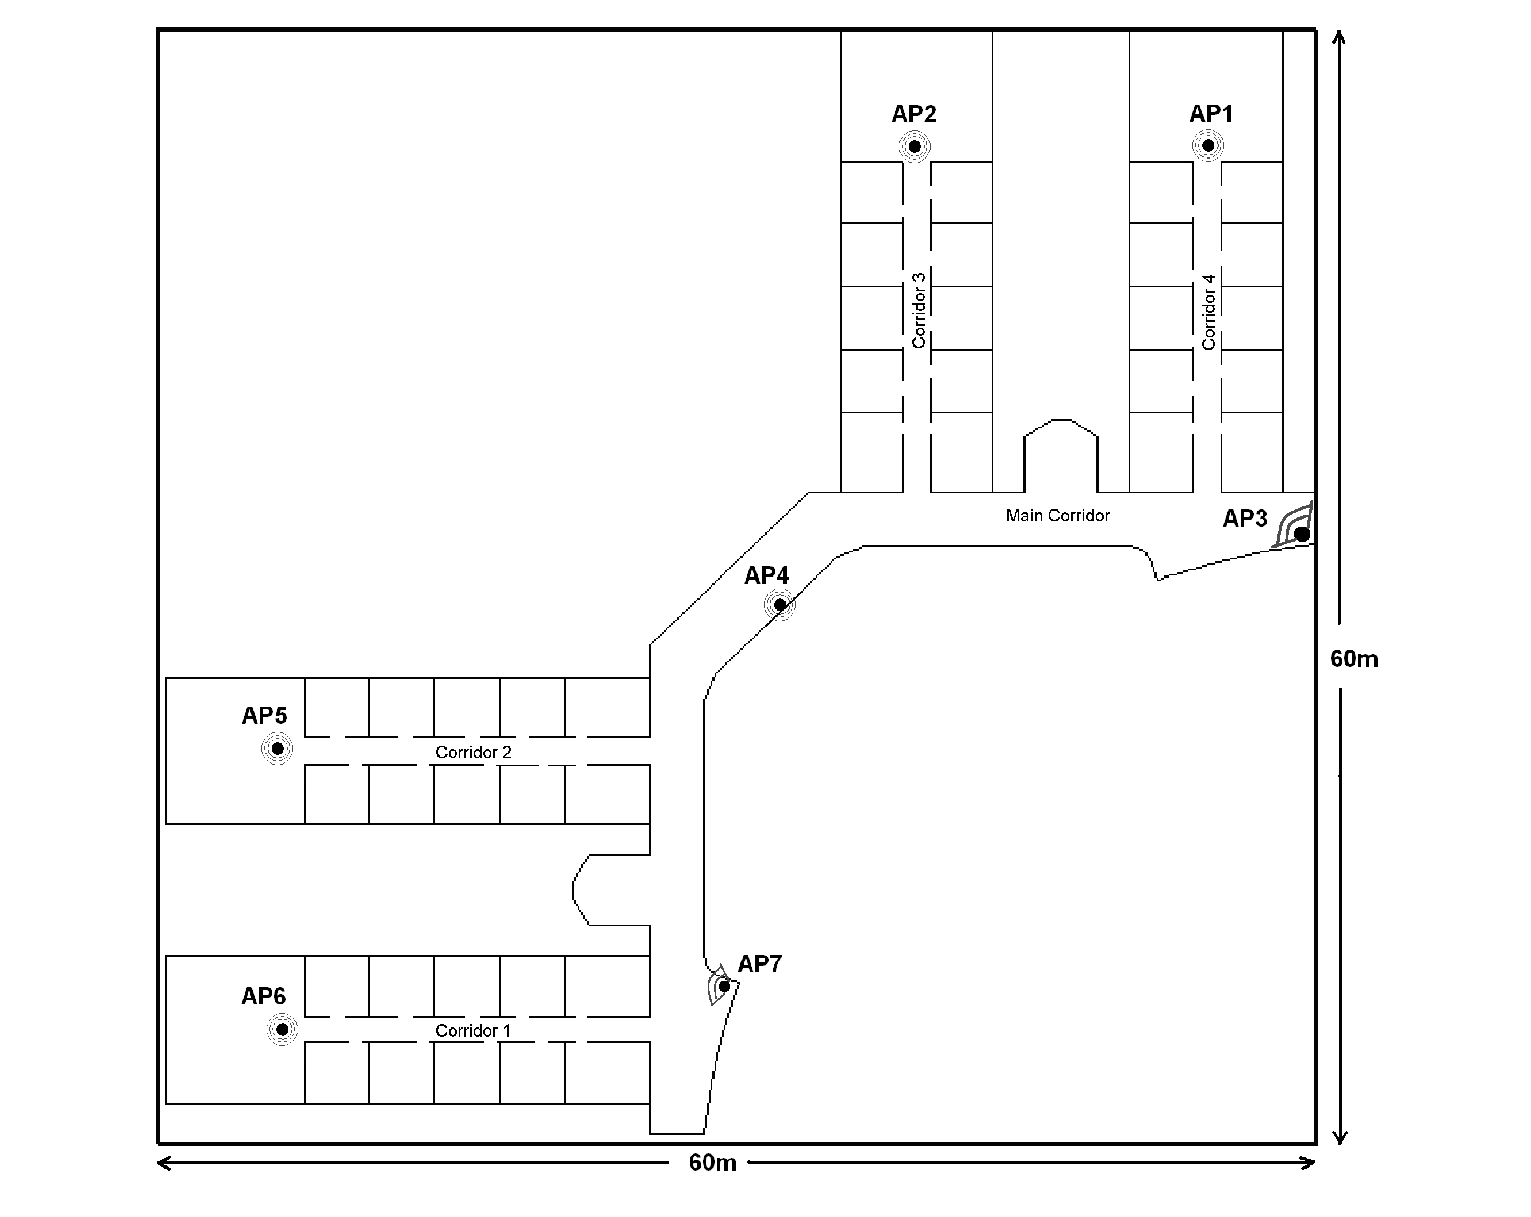
\includegraphics[width=0.4\textwidth]{Figure1}
    \caption{Ejemplo de figura con wrapfigure.}
    \label{fig:wrapfigure1}
  \end{center}
  \vspace{-20pt}
  \vspace{1pt}
\end{wrapfigure} 

Otra posibilidad es utilizar el entorno \texttt{wrapfig} para hacer que el texto bordee a las figuras, como en la figura~\ref{fig:wrapfigure1}. Añado ahora unas líneas de loren ipsum para que lo veáis bien. \lipsum[1-1]

% \lipsum[1-4]
% \begin{wrapfigure}{R}{5cm}
% \centering
% \rule{3cm}{7cm}
% \end{wrapfigure}
% \lipsum[1-6]

Incluso podemos poner una tabla ``apaisada'', como en la \ref{tab:tablas2006}, donde se muestra un resumen de los resultados obtenidos en una serie de experimentos de localización de locutores.

\clearpage
% \begin{table}[H]\centering
\begin{sidewaystable}[hbtp]
  \begin{center}

    \begin{tabular}{||l|c|c|c|c|c||}
      \hline \hline
      & UKA & ITC & AIT & UPC & IBM\\
      \hline
      \hline
      Pcor & $57.0\pm1.4\%$ & $84.0\pm3.3\%$ & $47.0\pm3.1\%$ & $20.0\pm2.5\%$ & $67.0\pm2.9\%$ \\
      \hline
      Bias fine (x:y:z) [mm] & $20:-42:-75$ & $45:27:-41$ & $-27:-77:-40$ & $-59:112:52$ & $91:-69:-38$ \\
      \hline
      Bias fine+gross (x,y,z) [mm] & $735:-93:-258$ & $67:439:-134$ & $17:-402:-118$ & $-141:255:39$ & $474:-141:-14$ \\
      \hline
      AEE fine [mm] = MOTP & $210$ & $130$ & $266$ & $344$ & $228$ \\
      \hline
      Fine+gross [mm] & $1201$ & $632$ & $1006$ & $1188$ & $884$ \\
      \hline
      Loc. frames & $5035$ & $22$ & $995$ & $977$ & $1023$ \\
      \hline
      Ref. duration (s) & $6287.0$ & $596.0$ & $1143.0$ & $1180.0$ & $1194.0$ \\
      \hline \hline
    \end{tabular}
    \caption{Resultados TEST CLEAR 2006.}
    \label{tab:tablas2006}
  \end{center}
\end{sidewaystable}
% \end{table}


\section{Conclusiones}
\label{sec:conclusiones-resultados}

Blah, blah, blah.


%%% Local Variables:
%%% TeX-master: "../book"
%%% End:


%%%%%%%%%%%%%%%%%%%%%%%%%%%%%%%%%%%%%%%%%%%%%%%%%%%%%%%%%%%%%%%%%%%%%%%%%%%
%
% Generic template for TFC/TFM/TFG/Tesis
%
% By:
%  + Javier Macías-Guarasa.
%    Departamento de Electrónica
%    Universidad de Alcalá
%  + Roberto Barra-Chicote.
%    Departamento de Ingeniería Electrónica
%    Universidad Politécnica de Madrid
%
% By: + Javier Macías-Guarasa. Departamento de Electrónica Universidad de Alcalá + Roberto Barra-Chicote. Departamento de Ingeniería Electrónica Universidad Politécnica de Madrid
% 
% Based on original sources by Roberto Barra, Manuel Ocaña, Jesús Nuevo, Pedro Revenga, Fernando Herránz and Noelia Hernández. Thanks a lot to all of them, and to the many anonymous contributors found (thanks to google) that provided help in setting all this up.
%
% See also the additionalContributors.txt file to check the name of additional contributors to this work.
%
% If you think you can add pieces of relevant/useful examples, improvements, please contact us at (macias@depeca.uah.es)
%
% You can freely use this template and please contribute with comments or suggestions!!!
%
%%%%%%%%%%%%%%%%%%%%%%%%%%%%%%%%%%%%%%%%%%%%%%%%%%%%%%%%%%%%%%%%%%%%%%%%%%%

\chapter{Conclusiones y líneas futuras}
\label{cha:concl-y-line}

En este apartado se resumen las conclusiones obtenidas y se proponen futuras líneas de investigación que se deriven del trabajo.

La estructura del capítulo es...


\section{Conclusiones}
\label{sec:conclusiones}

Para añadir una referencia a un autor, se puede utilizar el paquete \texttt{cite}. En el trabajo \cite{armani03}, se muestra un trabajo...

Y podemos usar de nuevo algún acrónimo, como por ejemplo \ac{TDPSOLA}, o uno ya referenciado como \ac{ANN} que cambia cuando lo usas una segunda vez \ac{ANN}.

Veamos finalmente si funciona una cita inline... al paper de Leticia \fullcite{monasterio2022}... (esto substituye la funcionalidad de bibentry...).


\section{Líneas futuras}
\label{sec:lineas-futuras}

Pues eso.


%%% Local Variables:
%%% TeX-master: "../book"
%%% End:




%%%%%%%%%%%%%%%%%%%%%%%%%%%%%%%%%%%%%%%%%%%%%%%%%%%%%%%%%%%%%%%%%%%%%%%%%%%%
%
% Generic template for TFC/TFM/TFG/Tesis
%
% $Id: pliego.tex,v 1.3 2013/11/25 00:33:32 macias Exp $
%
% By:
%  + Javier Mac�as-Guarasa. 
%    Departamento de Electr�nica
%    Universidad de Alcal�
%  + Roberto Barra-Chicote. 
%    Departamento de Ingenier�a Electr�nica
%    Universidad Polit�cnica de Madrid   
% 
% Based on original sources by Roberto Barra, Manuel Oca�a, Jes�s Nuevo,
% Pedro Revenga, Fernando Herr�nz and Noelia Hern�ndez. Thanks a lot to
% all of them, and to the many anonymous contributors found (thanks to
% google) that provided help in setting all this up.
%
% See also the additionalContributors.txt file to check the name of
% additional contributors to this work.
%
% If you think you can add pieces of relevant/useful examples,
% improvements, please contact us at (macias@depeca.uah.es)
%
% Copyleft 2013
%
%%%%%%%%%%%%%%%%%%%%%%%%%%%%%%%%%%%%%%%%%%%%%%%%%%%%%%%%%%%%%%%%%%%%%%%%%%%

\chapter{Pliego de condiciones}
\label{cha:pliego-de-condiciones}

Blah, blah, blah.

%%% Local Variables:
%%% TeX-master: "../book"
%%% End:


%\chapter{Presupuesto}
\label{cha:presupuesto}

Blah, blah, blah.


%%%%%%%%%%%%%%%%%%%%%%%%%%%%%%%%%%%%%%%%%%%%%%%%%%%%%%%%%%%%%%%%%%%%%%%%%%%
% Bibliography
%%%%%%%%%%%%%%%%%%%%%%%%%%%%%%%%%%%%%%%%%%%%%%%%%%%%%%%%%%%%%%%%%%%%%%%%%%%
%%%%%%%%%%%%%%%%%%%%%%%%%%%%%%%%%%%%%%%%%%%%%%%%%%%%%%%%%%%%%%%%%%%%%%%%%%%
%
% Generic template for TFC/TFM/TFG/Tesis
%
% $Id: bibliography.tex,v 1.6 2013/11/25 00:33:31 macias Exp $
%
% By:
%  + Javier Mac�as-Guarasa. 
%    Departamento de Electr�nica
%    Universidad de Alcal�
%  + Roberto Barra-Chicote. 
%    Departamento de Ingenier�a Electr�nica
%    Universidad Polit�cnica de Madrid   
% 
% Based on original sources by Roberto Barra, Manuel Oca�a, Jes�s Nuevo,
% Pedro Revenga, Fernando Herr�nz and Noelia Hern�ndez. Thanks a lot to
% all of them, and to the many anonymous contributors found (thanks to
% google) that provided help in setting all this up.
%
% See also the additionalContributors.txt file to check the name of
% additional contributors to this work.
%
% If you think you can add pieces of relevant/useful examples,
% improvements, please contact us at (macias@depeca.uah.es)
%
% Copyleft 2013
%
%%%%%%%%%%%%%%%%%%%%%%%%%%%%%%%%%%%%%%%%%%%%%%%%%%%%%%%%%%%%%%%%%%%%%%%%%%%

%\bibliographystyle{plainnat}
%\bibliographystyle{dinat}
%\bibliographystyle{unsrt}
\bibliographystyle{IEEEtran}
\bibliography{biblio/biblio}


%%% Local Variables:
%%% TeX-master: "../book"
%%% End:





%%%%%%%%%%%%%%%%%%%%%%%%%%%%%%%%%%%%%%%%%%%%%%%%%%%%%%%%%%%%%%%%%%%%%%%%%%%
% Appendices
%%%%%%%%%%%%%%%%%%%%%%%%%%%%%%%%%%%%%%%%%%%%%%%%%%%%%%%%%%%%%%%%%%%%%%%%%%%
% I don't recommend it, but if you want to define "parts", use this...
% BEWARE: I didn't write the english dependent code
%\part*{Ap�ndices}
%\label{part:apendices}

\appendix
%%%%%%%%%%%%%%%%%%%%%%%%%%%%%%%%%%%%%%%%%%%%%%%%%%%%%%%%%%%%%%%%%%%%%%%%%%%
%
% Generic template for TFC/TFM/TFG/Tesis
%
% $Id: manual.tex,v 1.3 2013/11/04 23:46:21 macias Exp $
%
% By:
%  + Javier Mac�as-Guarasa. 
%    Departamento de Electr�nica
%    Universidad de Alcal�
%  + Roberto Barra-Chicote. 
%    Departamento de Ingenier�a Electr�nica
%    Universidad Polit�cnica de Madrid   
% 
% Based on original sources by Roberto Barra, Manuel Oca�a, Jes�s Nuevo,
% Pedro Revenga, Fernando Herr�nz and Noelia Hern�ndez. Thanks a lot to
% all of them, and to the many anonymous contributors found (thanks to
% google) that provided help in setting all this up.
%
% If you think you can add pieces of relevant/useful examples,
% improvements, please contact us at (macias@depeca.uah.es)
%
% Copyleft 2013
%
%%%%%%%%%%%%%%%%%%%%%%%%%%%%%%%%%%%%%%%%%%%%%%%%%%%%%%%%%%%%%%%%%%%%%%%%%%%

\chapter{Manual de usuario}
\label{cha:concl-y-line}

\section{Introducci�n}
\label{sec:introapp1}


Introducci�n.

\section{Manual}
\label{sec:manual}

Pues eso.

\section{C�digo fuente}
\label{sec:codigo-fuente}

As� se inserta c�digo fuente.

\lstset{language=c++}
\lstset{tabsize=2}
\lstset{commentstyle=\textit}
\lstset{stringstyle=\ttfamily, basicstyle=\small}
\begin{lstlisting}[frame=trbl]{}
void funcionPrueba()
{	
	int prueba;
}
\end{lstlisting}


	

%%% Local Variables:
%%% TeX-master: "../book"
%%% End:




\chapter{Herramientas y recursos}
\label{cha:herr-y-recurs}

Las herramientas necesarias para la elaboraci�n del proyecto han sido:

\begin{itemize}
\item PC compatible 
\item Sistema operativo GNU/Linux \cite{gnulinux}
\item Entorno de desarrollo Emacs \cite{emacs}
\item Entorno de desarrollo KDevelop \cite{kdevelop}
\item Procesador de textos \LaTeX \cite{lamport94}
\item Lenguaje de procesamiento matem�tico Octave  \cite{octave}
\item Control de versiones CVS \cite{cvs}
\item Compilador C/C++ gcc \cite{gcc}
\item Gestor de compilaciones make \cite{make}
\end{itemize}


\backmatter

% Just fot TFGs at UAH
\ifthenelse{\boolean{tfguah}}
{
  \cleartoleftpage
\thispagestyle{plain}

% To add background watermark
\BgThispage

\begin{tikzpicture}[remember picture,overlay]

  draw[fill=headingPortadaTFM] (current page.north.west) rectangle -(\paperwidth,5cm);

\end{tikzpicture}

% Nice example of tikz
% \begin{tikzpicture}[remember picture,overlay]
%   \node [xshift=1cm,yshift=1cm] at (current page.south west)
%   [text width=7cm,fill=red!20,rounded corners,above right]
%   {
%     This is an absolutely positioned text in the
%     lower left corner. No shipout-hackery is used.
%   };
% \end{tikzpicture}

\begin{tikzpicture}[remember picture,overlay]
    \node[yshift=-5cm] at (current page.north west)
      {
        \begin{tikzpicture}[remember picture, overlay]
          \draw[fill=headingPortadaTFM] (0,0) rectangle (\paperwidth,5cm);
          \node [yshift=3cm, xshift=0.5\paperwidth, font=\Huge, text centered, midway] {\color{textoHeadingPortadaTFM}Universidad de Alcal�};
          \node [yshift=2cm, xshift=0.5\paperwidth, font=\Huge, text centered, midway] {\color{textoHeadingPortadaTFM}Escuela Polit�cnica Superior};

        \end{tikzpicture}
      };
   \end{tikzpicture}


\large
\vspace{20cm}
\begin{center}
  
  \centerline{\includegraphics[height=2.5cm]{logoUAH.jpg}}

\end{center}



}
{

}

\end{document}

